\chapter{End of chapter exercise solutions}
\label{eoceSolutions}



%_______________
\eocesolch{Introduction to data}



%_______________
\begin{multicols}{2}

%% 9.1 CASE STUDY: PREVENTING PEANUT ALLERGIES
	
% 1

\eocesol{(a)~Treatment: $10/43 = 0.23 \rightarrow 23\%$. \\
	Control: $2/46 = 0.04 \rightarrow 4\%$. \\
(b)~At first glance, it appears patients in the treatment group seem more 
likely to experience pain reduction from the acupuncture treatment. There is a 19\% difference between the pain reduction rates in the two 
groups, with the treatment group experiencing the higher pain reduction rate.}

% 2 

\eocesol{(a)~Treatment: $66/85 = 0.78 \rightarrow 78\%$ of patients in the treatment group experienced a significant improvement in symptoms. \\
	Control: $66/81 = 0.80 \rightarrow 80\%$ of patients in the control group experienced a significant improvement in symptoms. \\
	(b)~The control group's symptomatic treatments appear to be more effective than the treatment group's amoxicillin treatment because the control group has a higher percentage of patients who reported significant improvement in symptoms than the treatment group (80\% vs. 78\%). \\
	(c)~Answers may vary but should be sensible. Possible answer: Because the observed 2\% difference is rather small, the observed difference may well be simply due to chance.}


%% 9.2 DATA BASICS


% 3

\eocesol{(a)~143,196 eligible study subjects born in Southern California between 1989 
	and 1993. \\
	(b)~Measurements of carbon monoxide, nitrogen dioxide, ozone, and particulate 
	matter less than 10$\mu g/m^3$ (PM$_{10}$) collected at air-quality-monitoring 
	stations as well as length of gestation. Continuous numerical variables.  \\
	(c)~"Is there an association between air pollution 
	exposure and incidence of preterm births?"}

% 4

\eocesol{(a)~600 asthma patients, ages 18-69.  \\
	(b)~Scores on quality of life, activity, asthma symptoms, and medication reduction on a scale from 0 to 10. Ordinal categorical variables. \\
	(c)~"Is there evidence that the Buteyko method reduces asthma and improves quality of life?"}

% 5

\eocesol{(a)~The control tests are the ones in which hummingbirds are presented with either sucrose or water. The treatment tests are the ones in which hummingbirds are presented with test stimuli (aspartame, erythritol). \\
	(b)~Length of time a hummingbird drank from each of the two containers in a given trial. Numerical variable. \\
	(c)~"Does the T1R1-T1R3 taste receptor in hummingbirds play a role in detecting sweetness?"}

% 6

\eocesol{(a)~Control: the group of 16 female birds that received no treatment. Treatment: the group of 16 female birds that were given supplementary diets. \\
	(b)~"Does egg coloration indicate the health of female collared flycatchers?" \\
	(c)~Darkness of blue color in female birds' eggs. Continuous numerical variable.}

% 7

\eocesol{(a)~Each row represents a participant. \\
	(b)~1,691 participants. \\
	(c)~Sex: nominal categorical variable. Age: discrete numerical variable. Marital status: nominal categorical variable. Gross income: ordinal categorical variable. Smoking status: nominal categorical variable. Amount of smoking during weekends: discrete numerical variable. Amount of smoking during weekdays: discrete numerical variable.}


\textC{\end{multicols}
\newpage
\begin{multicols}{2}}

% 8

\eocesol{(a)~Each row represents a participant. \\
	(b)~The response variable is colon cancer stage. The explanatory variables are the abundance levels of the five bacterial species. \\
	(c)~Colon cancer stage: ordinal categorical variable. Abundance levels of bacterial species: continuous numerical variable.  }

% 9 

\eocesol{(a)~The population of interest consists of babies born in Southern California. The sample consists of the 143,196 babies born between 1989 and 1993 in Southern California. \\
	(b)~Assuming that the sample is representative of the population of interest, the results of the study can be generalized to the population. The findings cannot be used to establish causal relationships because the study was an observational study, not an experiment.}

% 10

\eocesol{(a)~The population of interest consists of asthma patients who rely on medication for asthma treatment. The sample consists of the 600 asthma patients ages 18-69 who participated in the study. \\
	(b)~The sample may not be representative of the population because study participants were recruited, an example of a convenience sample. Thus, the results of the study may not be generalizable to the population. The findings can be used to establish causal relationships because the study is an experiment conducted with control, randomization, and a reasonably large sample size.}


% 11

\eocesol{(a)~The population of interest consists of healthy young adults. The sample consists of the 437 healthy young adult volunteers from the University of Virginia. \\
	(b)~The sample may not be representative of the population because study participants were volunteers, an example of a convenience sample. Additionally, participants were all from the University of Virginia community; it is possible that there may be a systematic difference between these young adults and those in the wider population. Thus, the results may not be generalizable to the population. Even so, many studies rely on this kind of convenience sampling. \\
	c)~The findings can be used to establish causal relationships because the study is an experiment conducted with a control, randomization, and a reasonably large sample size.}

%% 9.3 DATA COLLECTION PRINCIPLES

% 12

\eocesol{(a)~Experiment. The researchers directly intervened and assigned treatments, manipulating the explanatory variable to examine changes in the response variable. \\
	(b)~The explanatory variable is the dose of Vitamin C taken at the onset of a cold. The response variables are cold duration and severity. \\
	(c)~Yes, there may be underlying differences between participants who choose to take the pill and participants who choose not to take the pill. The researcher's analysis may introduce confounding if it is only based on the participants who chose to take the pill.}

% 13

\eocesol{(a)~Experiment.  \\
	(b)~The treatment group consists of the individuals assigned to exercise twice a week. The control group consists of of the individuals instructed not the exercise. \\
	(c)~Yes. The blocking variable is age. \\
	(d)~The results of the study can be used to establish a causal relationship because the study is an experiment. Since the only systematic difference between the groups was the difference in the explanatory variable, it is reasonable to attribute the observed changes in the response variable to differences in the explanatory variable. The conclusions can be generalized to the larger population since the sample is representative of the population. \\
	(e)~Answers may vary. Possible answer: A more complex study design may be required in order to account for differences in participants' usual exercise habits. In the current design, individuals in the treatment group are simply instructed to exercise twice a week; for some, this could be an increase in exercise, and others, this could be a decrease. To address this issue, the treatment group participants could be instructed to exercise once a week more than usual, while the control group participants are instructed to maintain their current exercise regime. In the analysis, participants would need to be compared according to their initial exercise regimes.}

% 14

\eocesol{(a)~Experiment. \\
	(b)~The experimental group consists of the chicks that received vitamin supplements. The control group consists of the chicks that did not receive vitamin supplements. \\
	(c)~Randomization ensures that there are not systematic differences between the control and treatment groups. Even if chicks may vary in ways that affect body mass and corticosterone levels, random allocation essentially evens out such differences, on average, between the two groups. This is essential for a causal interpretation of the results to be valid.}

\textC{\end{multicols}
\newpage
\begin{multicols}{2}}

% 15

\eocesol{(a)~Observational study. \\
	(b)~Answers may vary. One possible confounding variable is the wealth of a country. A wealthy country's citizens tend to have a higher life expectancy due to a higher quality of life, and the country tends to have a higher percentage of internet users because there is enough money for the required infrastructure and citizens can afford computers. Wealth of a country is associated with both estimated life expectancy and percentage of internet users. Omitting the confounder from the analysis distorts the relationship between the two variables, such that there may seem to be a direct relationship when there is not.}

% 16

\eocesol{(a)~Observational study. \\
	(b)~No, observational studies can only establish correlation. \\
	(c)~Answers may vary. One possible confounding variable is final exam period. Final exam period may increase both student stress (students may study more and sleep less) and muscle cramps (students may be less active because they are studying).}

% 17 

\eocesol{(a)~Simple random sampling is reasonable if 500 students is a large enough sample size relative to the total student population of the university. \\
	(b)~Since student habits may vary by field of study, stratifying by field of study would be a reasonable decision. \\
	(c)~Students in the same class year may have more similar habits. Since clusters should be diverse with respect to the outcome of interest, this would not be a good approach.}

% 18

\eocesol{(a)~Non-responders may have a different response to this question, e.g. 
parents who returned the surveys likely don't have difficulty spending time 
with their children. \\
(b)~It is unlikely that the women who were reached at the same address 3 years 
later are a random sample. These missing responders are probably renters 
(as opposed to homeowners) which means that they might be in a lower socio-economic class than the respondents. \\
(c)~This is an observational study, not an experiment, so it is not advisable to draw conclusions about causal relationships. The relationship may be in the other direction; i.e., that these people go running precisely because they do not have joint problems. Additionally, the data are not even sufficient to provide evidence of an association between running and joint problems because data have only been collected from individuals who go running regularly. Instead, a sample of individuals should be collected that includes both people who do and do not regularly go running; the number of individuals in each group with joint problems can then be compared for evidence of an association.}

% 19

\eocesol{(a)~Effective. The random sample will likely be representative of the city. \\
	(b)~Effective. This method ensures that each neighborhood is represented in the sample. A feature of this sample is that each neighborhood will be represented by an equal number of households; this is not, however, necessarily reflective of neighborhood sizes in the city. In a simple random sample, households from smaller neighborhoods are less likely to be chosen, and vice versa for households from larger neighborhoods; this leads to a sample that is strictly representative of the population. \\
	(c)~Not effective. It seems likely that neighborhoods are more variable than the households within a single neighborhood; thus, it is inefficient to sample all the households in a selected neighborhood. \\
	(d)~Effective. This addresses the issue with the sampling strategy in (c). \\
	(e)~Not effective. The sample would not be representative of the city since households closer to the city council offices may share characteristics that households farther from the city do not have. This sampling method would result in a biased sample.}

% 20 

\eocesol{(a)~No. The study is an observational study, so only conclusions about correlation can be drawn. However, it is important to note that an experiment would not be ethical here. \\
	(b)~No, because it implies a causal relationship between sleep disorders and bullying. In this case, we can at most conclude that there is a correlation between symptoms of sleep disorders and bullying in school children.}

% 21 

\eocesol{The lead author's statements are not accurate because he or she drew conclusions about causation (that increased alcohol sales taxes lower rates of sexually transmitted infections) from an observational study. In addition, although the study observed that there was a decline in gonorrhea rate, the lead author generalized the observation to all sexually transmitted infections.}


\textC{\end{multicols}
\newpage
\begin{multicols}{2}}

%% 9.4 NUMERICAL DATA

% 22
\eocesol{(a)~The two distributions have the same median since they have the same middle number when ordered from least to greatest. Distribution 2 has a higher IQR because its first and third quartiles are farther apart than in Distribution 2. \\
	(b)~Distribution 2 has a higher median since it has a higher middle number when ordered from least to greatest. Distribution 2 has a higher IQR because its first and third quartiles are farther apart than in Distribution 1. \\
	(c)~Distribution 2 has a higher median since all values in this distribution are higher than in Distribution 1. The two distributions have the same IQR since the distance between the first and third quartiles in each distribution is the same. \\
	(d)~Distribution 2 has a higher median since most values in this distribution are higher than those in Distribution 1. Distribution 2 has a higher IQR because its first and third quartiles are farther apart than those of Distribution 1.}

% 23

\eocesol{(a)~Distribution~2 has a higher mean since $20 > 13$, and a higher standard deviation 
since 20 is further from the rest of the data than 13. \\
(b)~Distribution~1 has a higher mean since $-20 > -40$, and Distribution~2 has a 
higher standard deviation since -40 is farther away from the rest of the data than -20. \\
(c)~Distribution~2 has a higher mean since all values in this distribution are higher 
than those in Distribution~1, but both distribution have the same standard deviation 
since they are equally variable around their respective means. \\
(d)~Both distributions have the same mean since they are both centered at 300, but 
Distribution~2 has a higher standard deviation since the observations are farther from 
the mean than in Distribution~1.}

% 24

\eocesol{(a)~Symmetric, centered at 60. Boxplot 2.
	(b)~Symmetric, centered at 50. Boxplot 3.
	(c)~Right skew, centered at 1. Boxplot 1.}

% 25

\eocesol{(a)~The distribution is bimodal, with peaks between 15-20 and 25-30. Values range from 0 to 65.  \\
(b)~The median AQI is about 30. \\
(c)~I would expect the mean to be higher than the median, since there is some right skewing.}

% 26 

\eocesol{(a)~Symmetric. There are no outliers; the boxplot does not show points outside the range of the whiskers. \\
	(b)~ Answers may vary. The histogram is more informative because it provides a more detailed picture of how the data are distributed, while the boxplot does not provide information about the overall shape of the distribution. Alternatively, the boxplot more clearly shows the median and interquartile range. \\
	(c)~Answers may vary. Various factors could influence the number of elderly people in a given state who choose to live in nursing homes. In states that are more sparsely populated, more residents might choose to stay in nursing homes because of the difficulties associated with living in rural areas, such as absence of easily accessible medical care. In wealthier states, however, people are less likely to live in nursing homes because of their ability to afford the costs of staying home (e.g. in-home nursing care); Social Security, Medicare, and Medicaid pay quite a lot of nursing home costs.}

% 27

\eocesol{(a)~The distribution of the scores show right skew. The scores range from 0 to about 18, with the majority of scores under 10. \\
	(b)~Since the distribution is skewed, the robust measures of center and spread, median and IQR, provide a better summary of the data.}

% 28

\eocesol{No, the midrange is sensitive to outliers and extreme skew since it is calculated using the two most extreme values in the distribution. If the extreme values in the distribution change, then the midrange will change, even if the rest of the distribution did not change.}

%% 9.5 CATEGORICAL DATA

% 29

\eocesol{(a)~Conservatives: 372/910 = 0.41 $\rightarrow$ 41\% \\
	(b)~In favor of the citizenship option: 278/910 = 0.31 $\rightarrow$ 31\% \\
	(c)~Conservative and in favor of the citizenship option: 57/910 = 0.06 $\rightarrow$ 6\% \\
	(d)~In favor of the citizenship option among conservatives: 57/372 = 0.15 $\rightarrow$ 15\% 
	In favor of the citizenship option among moderates: 120/363 = 0.33 $\rightarrow$ 33\%
	In favor of the citizenship option among liberals: 101/175 = 0.58 $\rightarrow$ 58\%}

% 30

\eocesol{(a)~These data are categorical. They can be summarized numerically in either a frequency table or relative frequency table, and summarized graphically in a bar plot of either counts or proportions. \\
	(b)~The results of these studies cannot be generalized to the larger population. Individuals taking the survey represent a specific subset of the population that are conscious about dental health, since they are at the dentist's office for an appointment. Additionally, there may be response bias; even though the surveys are anonymous, it is likely that respondents will feel some pressure to give a "correct" answer in such a setting, and claim to floss more often than they actually do.}

\textC{\end{multicols}
\newpage
\begin{multicols}{2}}

%% 9.6 RELATIONSHIPS BETWEEN TWO VARIABLES

% 31

\eocesol{(a)~Yes, there seems to be a positive association between lifespan and length of gestation. Generally, as gestation increases, so does life span. \\
	(b)~Positive association. Reversal of the plot axes does not change the nature of an association.}

% 32

\eocesol{(a)~Plot 1, linear. Plot 3, nonlinear.
	(b)~Plot 4, linear.
	(c)~Plot 2.}

% 33

\eocesol{(a)~75\% of the countries have an adolescent fertility rate less than or equal to 75.73 births per 1,000 adolescents. \\
	(b)~It is likely that the observations are missing due to the Iraq War and general instability in the region during this time period. It is unlikely that the five-number summary would have been affected very much, even if the values were extreme; the median and IQR are robust estimates, and the dataset is relatively large, with data from 188 other countries. \\
	(c)~The median and IQR decreases each year, with Q1 and Q3 also decreasing.}

% 34 

\eocesol{(a)~51/215 = 0.24 $\rightarrow$ 24\% of the participants were both smokers and had aortic stenosis. The other three numbers of the joint distribution are: 54/215 = 0.25 $\rightarrow$ 25\% (percent of participants who were smokers and did not have aortic stenosis); 43/215 = 0.20 $\rightarrow$ 20\% (percent of participants who were non-smokers and had aortic stenosis); and 67/215 = 0.31 $\rightarrow$ 31\% (percent of participants who were non-smokers and did not have aortic stenosis). \\
	(b)~Among the 105 smokers, 51 have aortic stenosis. Thus, 51/105 of the smokers have aortic stenosis. Among the 110 non-smokers, 43 have aortic stenosis. Thus, 43/110 of the non-smokers have aortic stenosis. \\
	(c)~The relative risk of aortic stenosis, comparing smokers to non-smokers, is $\frac{51/105}{43/110} = 1.24$. The risk of a smoker developing aortic stenosis is 1.24 times that of a non-smoker. Since the relative risk is greater than 1, there does seem to be evidence that smoking is associated with an increased probability of stenosis. The relative risk is also greater than 1.2, indicating that a smoker's probability of stenosis is alarmingly higher than that of a non-smoker.}

% 35

\eocesol{(a)~4,371/8,474 = 0.56 $\rightarrow$ 56\% \\
	(b)~110/190 = 0.58 $\rightarrow$ 58\% \\
	(c)~27/633 = 0.04 $\rightarrow$ 4\% \\
	(d)~53/3,110 = 0.02 $\rightarrow$ 2\% \\
	(e)~Relative risk: $\frac{27/633}{53/3,110} = 2.50$. Yes, since the relative risk is greater than 1. A relative risk of 2.50 indicates that individuals with high trait anger are 2.5 times more likely to experience a CHD event than individuals with low trait anger. \\
	(f)~Side-by-side boxplots, since blood cholesterol level is a numerical variable and anger group is categorical.}

%_______________
\end{multicols}


\textC{\newpage}



%_______________
\eocesolch{Probability}

%% 2.1 DEFINING PROBABILITY

%_______________
\begin{multicols}{2}

% 1

\eocesol{(a)~False. These are independent trials. \\
(b)~False. There are red face cards. \\
(c)~True. A card cannot be both a face card and an ace.}

% 2

\eocesol{(a)~0. It is impossible to roll a pair of dice and get a sum of one. The smallest possible sum is 2 (1 and 1). \\
	(b)~$\frac{4}{36}$. There are 4 possible pairs sum to 5 (1 and 4; 2 and 3; 3 and 2; 4 and 1) and a total of 36 possible pairs (6 x 6), giving a probability of $\frac{\text{number of pairs that sum to 5}}{\text{total number of pairs}}$ = $\frac{4}{36}$. \\
	(c)~$\frac{1}{36}$. There is one possible pair that sums to 12 (6 and 6) and a total of 36 possible pairs (6 x 6), giving a probability of $\frac{\text{number of pairs that sum to 12}}{\text{total number of pairs}}$ = $\frac{1}{36}$.}

% 3

\eocesol{(a)~$\frac{1}{4}$. \\
	Solution 1: A colorblind male has genotype $X^{-}Y$. He must have inherited $X^{-}$ from his mother (probability of $\frac{1}{2}$) and $Y$ from his father (probability of $\frac{1}{2}$). Since these are two independent events, the probability of both occuring is $(\frac{1}{2}) (\frac{1}{2}) = \frac{1}{4}$. \\
	Solution 2: Determine the possibilities using a Punnett square. There are 4 equally likely possibilities, one of which is a colorblind male. Thus, the probability is $\frac{1}{4}$. 
	
	\begin{center}
		\begin{tabular}{ |c|c|c| } 
			\hline
			& $X^{+}$ & $Y$ \\ 
			\hline
			$X^{+}$ & $X^{+}X^{+}$ & $X^{+}Y$ \\ 
			\hline
			$X^{-}$ & $X^{+}X^{-}$ & $X^{-}Y$ \\ 
			\hline
		\end{tabular}
	\end{center}
	(b)~True. An offspring of this couple cannot be both female and colorblind.}

% 4

\eocesol{(a)~No. Someone can have diabetes and hypertension. \\
	(b)\\
	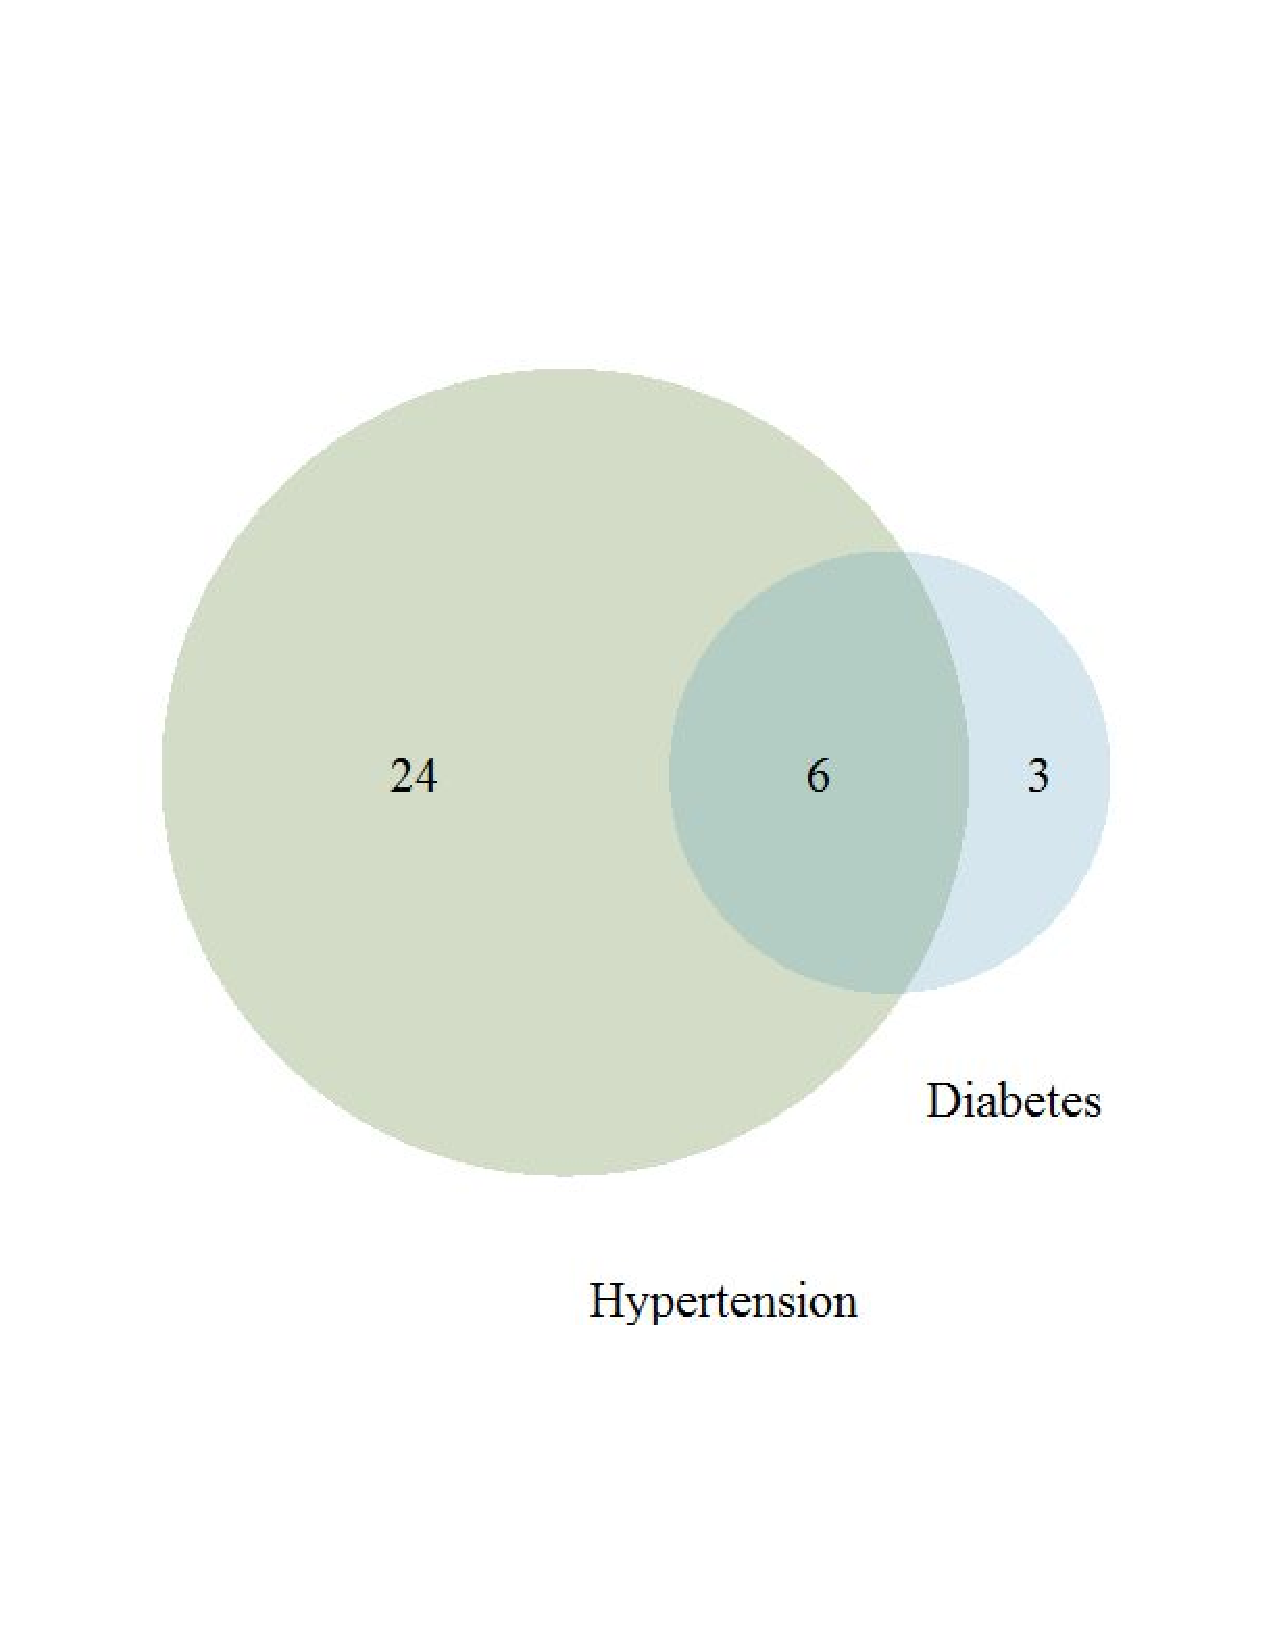
\includegraphics[width=40mm]{ch_probability_oi_biostat/figures/eoce/diabetes_hypertension/diabetes_hypertension.pdf} \\
	(c)~0.33. $P(\text{$A$ or $B$}) = P(A) + P(B) - P(\text{$A$ and $B$}) = 0.09 + 0.30 - 0.06 = 0.33$. \\
	(d)~67\%. $P(\text{$A^{C}$ and $B^{C}$}) = 1 - P(\text{$A$ or $B$}) = 1 - 0.33 = 0.67 = 67\%$. \\
	(e)~No. If diabetes (A) and hypertension (B) were independent, $P(\text{$A$ and $B$}) = P(A)P(B)$. Since $0.06 \neq (0.09)(0.30)$, i.e. $P(\text{$A$ and $B$}) \neq P(A)P(B)$, the events are not independent.}

% 5

\eocesol{(a)~No. Someone can live below the poverty line and speak a foreign language at home. \\
	(b)
	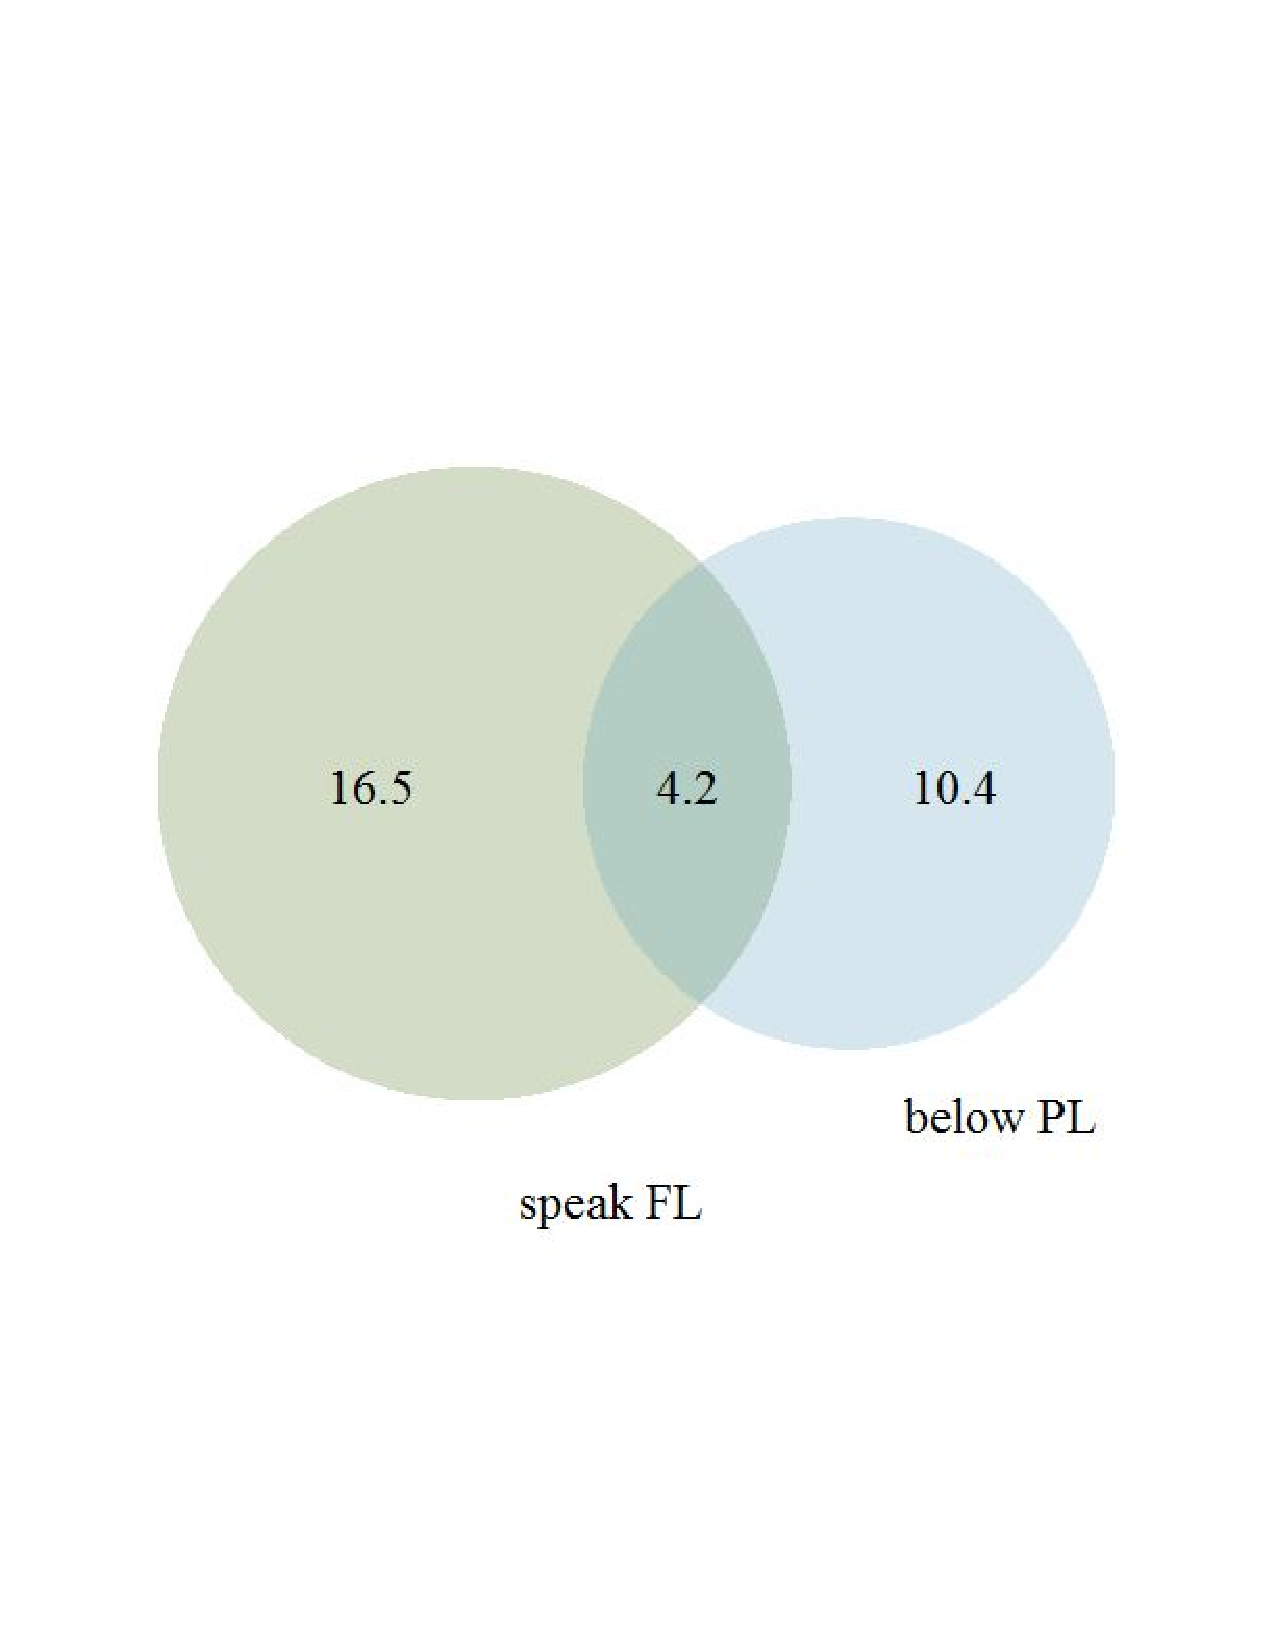
\includegraphics[width=40mm]{ch_probability_oi_biostat/figures/eoce/poverty_language/poverty_language.pdf} \\
	(c)~10.4\%. \\
	Solution 1: The "10.4\%" portion of the Venn diagram represents Americans who live below the poverty line and do not speak a foreign language at home (i.e. only speak English at home).
	Solution 2: Let $A$ = \{living below the poverty line\} and $B$ = \{speaking a foreign language at home\}. Given $P(A) = 0.146$, $P(B) = 0.207$, and $P(A \textrm{ and }B) = 0.042$, calculate $P(A \textrm { and } B^C)$. $P(A \textrm{ and }B^C) = P(A)P(B^C | A) = P(A)(1 - P(B|A)) = P(A)(1 - \frac{P(A \textrm{ and } B)}{P(A)}) = (0.146)(1 - \frac{0.042}{0.146}) = 0.104 \rightarrow 10.4\%$  \\
	(d)~31.1\%. $P(A \textrm{ or } B) = P(A) + P(B) - P(A \text{ and } B) = 0.146 + 0.207 - 0.042 = 0.311 \rightarrow 31.1\%$. \\
	(e)~68.9\%. The group of Americans who live above the poverty line and only speak English at home is represented in the Venn diagram by the space in the rectangle but outside either of the two circles. $P(A^{C} \text{ and } B^{C}) = 1- P(A \text{ or } B) = 1- 0.311 = 0.689 = 68.9\%$. \\
	(f)~No. If $A$ and $B$ were independent events, then $P(\text{$A$ and $B$}) = P(A)P(B)$. Since $0.042 \neq (0.146)(0.207)$, i.e. $P(\text{$A$ and $B$}) \neq P(A)P(B)$, the events are not independent.
	}
	
\textC{\end{multicols}
\newpage
\begin{multicols}{2}}

% 6 

\eocesol{(a)~0.25. Let $H$ represent the event of being a high school graduate and $F$ represent the event of being a woman. $P(H) = P(H \textrm{ and } W) + P(H \textrm{ and } W^C) = P(H|W)P(W) + P(H|W^C)P(W^C) = (0.20)(0.50) + (0.30)(0.50) = 0.25$. \\
	(b)~0.91.$(A^C) = P(A^C \textrm{ and } W) + P(A^C \textrm{ and } W^C) = (1-0.09) + (1-0.09) = 0.91$. \\
	(c)~0.25. Let $X$ represent the event of having at least a Bachelor's degree, where $B$ represents the event of attaining at most a Bachelor's degree and $G$ the event of attaining at most a graduate or professional degree.  $P(X|W^C) = P(B|W^C) + P(G|W^C) = 0.16 + 0.09 = 0.25$. \\
	(d)~0.26. $P(X|W) = P(B|W) + P(G|W) = 0.17 + 0.09 = 0.26$. \\
	(e)~0.065. Let $X_W$ be the event that a woman has at least a Bachelor's degree, and $X_M$ be the event that a man has at least a Bachelor's degree. Assuming that the education levels of the husband and wife are independent, $P(X_W \textrm{ and } X_M) = P(X_W) \times P(X_M) = (0.25)(0.26) = 0.065$. This assumption is probably not reasonable, because people tend to marry someone with a comparable level of education.
}

% 7 

\eocesol{(a)~0.32. Let $D_0$, $D_1$, $D_2$, $D_3$ represent the events of missing 0, 1, 2, and 3 or more days of school per year. $P(D_0) = 1 - P(D_0^C) = 1 - (P(D_1) + P(D_2) + P(D_3)) = 1- (0.25 + 0.15 + 0.28) = 0.32$. \\
	(b)~0.57. The probability of missing at most 1 day is equal to missing either 0 days or 1 day: $P(D_0) + P(D_1) = 0.32 + 0.25 = 0.57$.\\
	(c)~0.68. The probability of missing at least 1 day is equal to missing either 1, 2, or 3 or more days: $P(D_1) + P(D_2) + P(D_3) = 0.25 + 0.15 + 0.28.$. This can also be thought of as the complement of missing 0 days: $1 - P(D_0) = 1 - 0.32 = 0.68$.\\
	(d)~0.10. Assuming that the school attendance of one child is independent of that of the other child, $P(D_0) \times P(D_0) = (0.32)(0.32) = 0.10$. This assumption is probably not reasonable because the attendance of children from the same household is typically correlated. For example, the two children may have a parent that takes them to school at the same time. \\
	(e)~0.46. Assuming that the school attendance of one child is independent of that of the other child, $(0.68)(0.68) = 0.46$. This assumption is probably not reasonable because the attendance of children from the same household is typically correlated. For example, if one child becomes ill and cannot go to school, it is likely that the other child will also be ill and cannot go to school.}

% 8 

\eocesol{(a)~Let $C$ represent the event that one urgent care center sees 300-449 patients in a week. Assuming that the number of patient visits are independent between urgent care centers in a given county for a given week, the probability that three random urgent care centers see 300-449 patients in a week is $[P(C)]^3 = (0.288)^3 = 0.024$. This assumption is not reasonable because a county is a small area with relatively few urgent care centers; if one urgent care center takes in more patients than usual during a given week, so might other urgent care centers in the same county (e.g., this could occur during flu season). \\
	(b)~$2.32 \times 10^{-7}$. Let $D$ represent the event that one urgent care center sees 450 or more patients in a week. Assuming independence, the probability that 10 urgent care centers throughout a state all see 450 or more patients in a week is $[P(D)]^{10} = (0.217)^{10} = 2.32 \times 10^{-7}$. This assumption is reasonable because a state is a large area that contains many urgent care centers; the number of patients one urgent care center takes in is likely independent of the number of patients another urgent care center in the state takes in. \\
	(c)~No, it is not possible, because it is not reasonable to assume that the patient visits for a given week are independent of those for the following week.}


% 9

\eocesol{(a)~$459/20,000 = 0.023$. \\
	(b)~Let $A$ be the event of having excellent health and $B$ be the event of not having health coverage. $P(A \textrm{ or } B) = P(A) + P(B) - P(A \textrm{ and } B) = \frac{4,657}{20,000} + \frac{2,524}{20,000} - \frac{459}{20,000} = \frac{6,722}{20,000} = 0.336$. }


% 10

\eocesol{(a)~$0.60 + 0.20 - 0.18 = 0.62$ \\
	(b)~$0.18/0.20 = 0.90$ \\
	(c)~$0.11/0.33 = 0.33$ \\
	(d)~No, because the answers to parts (c) and (d) are not equal. If global waring belief were independent of political party, then among liberal Democrats and conservative Republicans, there would be equal proportions of people who believe the earth is warming. \\
	(e)~$0.06/0.34 = 0.18$ }



\textC{\end{multicols}
\newpage
\begin{multicols}{2}}

%% 2.1 CONDITIONAL PROBABILITY

% 11 (oi biostat)

\eocesol{(a)~0.25. Each parent can pass on either an A allele or a B allele with probability 0.5. For a child to have Group A blood, they must inherit an A allele from both parents. Alleles are inherited independently, thus, the probability of a child of this couple having Group A blood is $(0.50) \times (0.50) = 0.25$. \\
	(b)~0.141. The probability that one child has Type O blood is $(0.50) \times (0.50) = 0.25$, since the child must inherit the $i$ allele from both parents. The probability that a child does not have Type O blood is $1 - 0.25 =0.75$ (the complement). Each child inheriting alleles is an independent event. The probability that their first child has Type O blood and the next two do not is: $(0.25) \times (0.75) \times (0.75) = 0.141$. \\
	(c)~1/3. The event that one child has Type O blood and two do not can happen three distinct ways: either the first, second, or third child is the one child with Type O blood. Neither child is more or less likely to have Type O blood, so the conditional probability that it is the first child given the stated condition equals $1/3$ by symmetry. This can also be approached algebraically; let $A$ be the event that the first child has Type O blood and $B$ be the event that one child has Type O blood and two do not.
	\[P(A|B) = \dfrac{P(A \cap B)}{P(B)} = \dfrac{(0.25)(0.75)(0.75)}{(3)(0.25)(0.75)(0.75)} = \dfrac{1}{3} \] }

% 12

\eocesol{(a)~No. Someone can be in excellent health and have health coverage. \\
	(b)~0.2329. \\
	(c)~$0.2099/0.8738 = 0.2402$. \\
	(d)~$0.0230/0.1262 = 0.1823$. \\
	(e)~No. let $A$ represent the event of being in excellent health and $B$ represent the event of having health coverage. Under independence, $P(A \textrm{ and }B ) = P(A)P(B)$. Since $0.2099 \neq (0.2329)(0.8738)$, the events are not independent.}

% 13
\eocesol{(a)~$375,264/436,968 = 0.859$ \\
	(b)~$229,246/255,980 = 0.896$ \\
	(c)~0.896. This is equivalent to (b). \\
	(d)~$146,018/180,988 = 0.807$ \\
	(e)~$4,719/7,394 = 0.638$ \\
	(f)~No, because the answers to (c) and (d) are not equal. If gender and seat belt usage were independent, then among males and females, there would be the same proportion of people who always wear seat belts.}

% 14

\eocesol{(a)~$\frac{114 + 108 - 78}{204} = \frac{144}{204} = 0.706$. \\
	(b)~$\frac{78}{114} = 0.684$. \\
	(c)~$19/54 = 0.352$. $11/36 = 0.306$. \\
	(d)~No, because the answers to (b) and (c) are not equal. If the male respondents' eye colors were independent of their partners' eye colors, then among male respondents with blue eyes, brown eyes, and green eyes, there would be the same proportion who have partners with blue eyes.}

% 15 (oi, edited)

\eocesol{(a)~0.6049. \\ $P(D|T^{+}) = 
	\frac{P(T^{+}|D)P(D)}{P(T^{+}|D)P(D) + P(T^{+}|D^C)P(D^C)} = \\ \frac{(0.99)(0.03)}{(0.99)(0.03) + (1-0.98)(1-0.03)} = 0.6049$. \\
	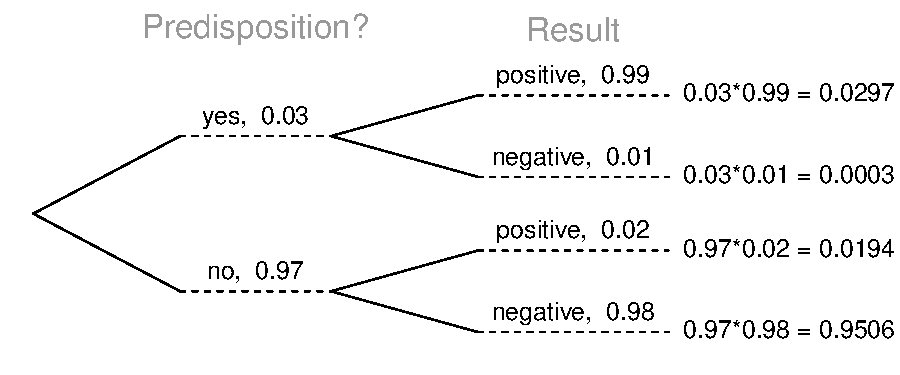
\includegraphics[width=60mm]{ch_probability_oi_biostat/figures/eoce/tree_thrombosis/tree_thrombosis.pdf}
	(b)~0.9994. \\ $P(D^C|T^{-}) = 
	\frac{P(T^{-}|D^C)P(D^C)}{P(T^{-}|D^C)P(D^C) + P(T^{-}|D)P(D)} = \\ \frac{(0.98)(1-0.03)}{(0.98)(1-0.03) + (1-0.99)(0.03)} = 0.9994$. \\}

% 16 (oi, edited)
\eocesol{The PPV is 0.8248. The NPV is 0.9728. \\ $P(D|T^{+}) = 
	\frac{P(T^{+}|D)P(D)}{P(T^{+}|D)P(D) + P(T^{+}|D^C)P(D^C)} = \\ \frac{(0.997)(0.0259)}{(0.997)(0.0259) + (1-0.926)(1-0.259)} = 0.8248$. \\
	\\ $P(D^C|T^{-}) = 
	\frac{P(T^{-}|D^C)P(D^C)}{P(T^{-}|D^C)P(D^C) + P(T^{-}|D)P(D)} = \\ \frac{(0.926)(1-0.259)}{(0.926)(1-0.259) + (1-0.997)(0.259)} = 0.9728$. \\
	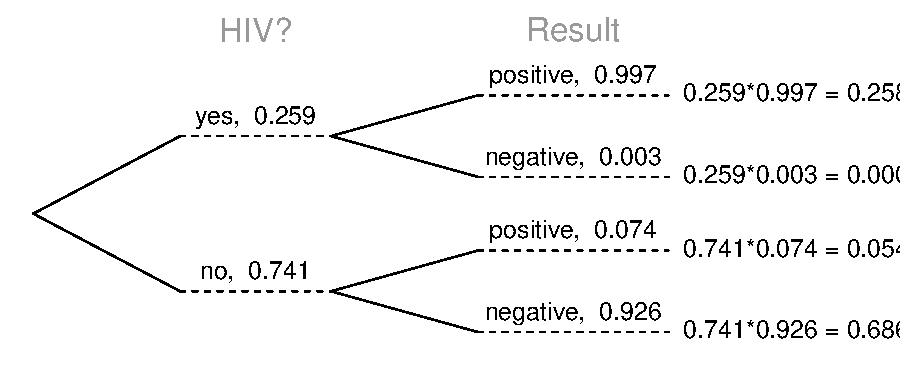
\includegraphics[width=60mm]{ch_probability_oi_biostat/figures/eoce/tree_hiv_swaziland/tree_hiv_swaziland.pdf}}

% 17

\eocesol{(a)~Let $E$ represent the event of agreeing with the idea of evolution and $D$ be the event of being a Democrat. From the problem statement, $P(E|D) = 0.67$. $P(E^C|D) = 1 - P(E|D) = 1 - 0.67 = 0.33$. \\
	(b)~Let $I$ represent the event of being an independent. $P(E|I) = 0.65$, as stated in the problem. \\
	(c)~Let $R$ represent the event of being a Republican. $P(E|R) = 1 - P(E^C|R) = 1 - 0.48 = 0.52$. \\
	(d)~0.35. $P(R|E) = \frac{P(E \textrm{ and }R)}{P(E)} = \frac{P(R)P(E|R)}{P(E)} = \frac{(0.40)(0.52)}{0.60} = 0.35$.}

\textC{\end{multicols}
\newpage
\begin{multicols}{2}}

% 18

\eocesol{(a)~Approximately 1,025 individuals would be expected to test positive; with approximately 25 true positive test results. The PPV of IRT is 0.0243.
	\\ $(100,000) P(T^+) = 100,000 [P(T+|D)P(D) + P(T|D^C)P(D^C)] = 100,000 [(0.87)(1/3500) + (1-0.99)(3499/3500)] \approx 1,025$. \\
	$(100,000) P(T^+|D) = (100,000)(0.87)(1/3500) \approx 25$. 
	$PPV \approx \frac{\textrm{\# true positives tests}}{\textrm{\# positive tests}} = 0.0243$. \\
	(b)~The PPV of IRT/IRT is 0.6839. Among the 1,025 individuals who tested positive in the first test, $25/1,025 = 0.0243$ are true positives; this represents the 'prevalence' of the group that undergo a second test. Recalculate PPV with the same test parameters: \\
	$PPV = \frac{P(T^+|D)P(D)}{P(T^+|D)P(D) + P(T^+|D^C)P(D^C)} = \\ \frac{(0.87)(0.0243)}{(0.87)(0.0243) + (1-0.99)(1-0.0243)} = 0.6839$.}

% 19

\eocesol{0.0714. Even when a patient tests positive for lupus, there is only a 7.14\% 
chance that he actually has lupus. House may be right.
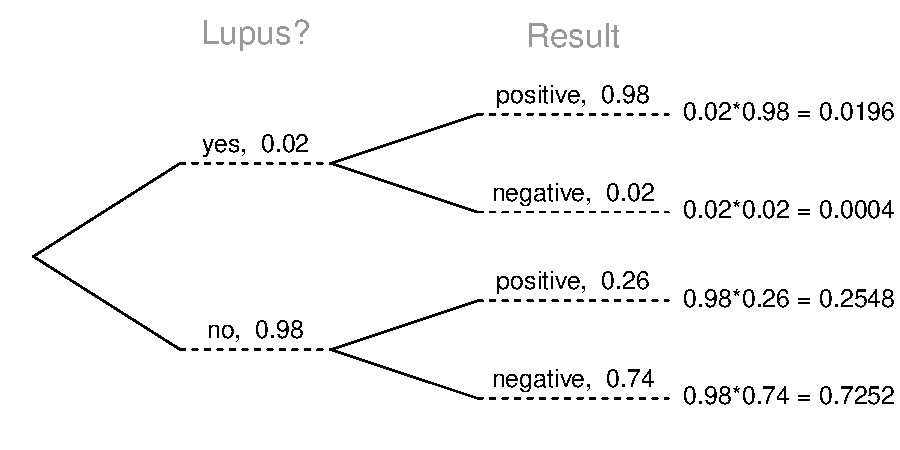
\includegraphics[width=60mm]{ch_probability_oi_biostat/figures/eoce/tree_lupus/tree_lupus.pdf}}


% 20

\eocesol{0.46. Let $I$ be the event of being identical twins, and $I^C$ be the event of being fraternal twins. Let $FF$ be the event that both twins are female. $P(I|FF) = \frac{P(I \textrm{ and } FF)}{P(FF)} = \frac{P(FF|I)P(I)}{P(FF|I)P(I) + P(FF|I^C)P(I^C)} = \frac{(0.50)(0.30)}{(0.50)(0.30) + (0.25)(1-0.30)} = 0.46$.\\
	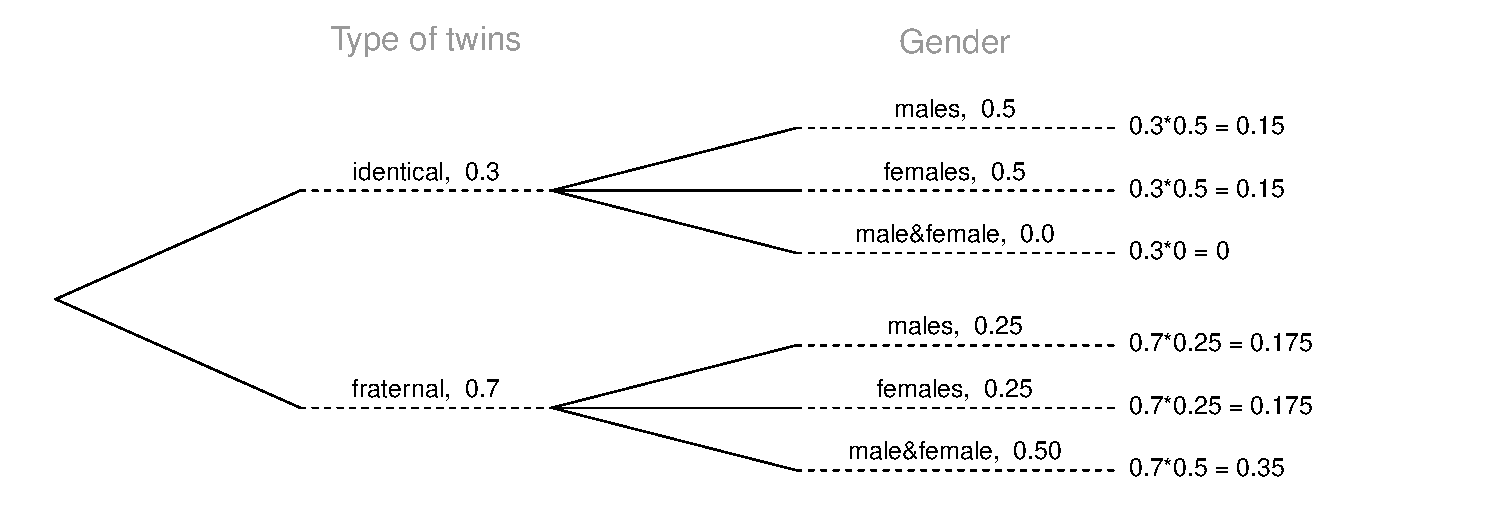
\includegraphics[width=60mm]{ch_probability_oi_biostat/figures/eoce/tree_twins/tree_twins.pdf}}

% 21

\eocesol{Mumps is the most likely disease state, since $P(B_3|A) = 0.563$, $P(B_1|A) = 0.023$, and $P(B_2|A) = .415$. $P(B_i|A) = \frac{P(A|B_i)P(B_i)}{P(A)}$. $P(A) = P(A \textrm{ and } B_1) + P(A \textrm{ and } B_2) + P(A \textrm{ and } B_3) = P(A|B_1)P(B_1) + P(A|B_2)P(B_2) + P(A|B_3)P(B_3)$. \\} 


% 22

\eocesol{(a)~In descending order on the table, the PPV for each age group is 0.070, 0.202, 0.293, 0.386, 0.403. As the prevalence of breast cancer increases, PPV also increases. If more women have the disease, the chance of a positive test result being a true positive increases (and the chances of the result being a false positive decreases). \\
	Consider the denominator, which quantifies the number of true positives and false positives. When prevalence increases, even though both the numerator and denominator are increasing from $[prev \times sensitivity]$, the denominator is also decreasing from $[(1-prev) \times (1-specificity)]$ decreasing (since as prevalence increases, the quantity $(1 - prev)$ decreases). Since sensitivity and specificity are constant, increasing prevalence has the effect of increasing the number of true positives (left term) and decreasing the number of false positives (right term). PPV increases when the number of true positives increases. \\
	(b)~ The technology that raises specificity to 99\% offers a higher increase. Since prevalence of the disease only ranges between less than 1\% to at most $\sim$ 4\%, most of the people tested do not have breast cancer. This implies that the low PPV is largely due to the high number of false positives. This value is related to the specificity. If specificity increases, this increases the number of true negatives and decreases the number of false positives. Increasing sensitivity can potentially increase the number of true positives detected and raise PPV, but this does not have as strong an effect.}

% 23 (oi_biostat)

\eocesol{(a)~Let $A$ be the event of knowing the answer and $B$ be the event of answering it correctly. Assume that if a participant knows the correct answer, they answer correctly with probability 1: $P(B|A) = 1$. If they guess randomly, they have 1 out of $m$ chances to answer correctly, thus $P(B|A^C) = 1/m$. $P(A|B)= \frac{1 \cdot p}{(1 \cdot p) +(\frac{1}{m} \cdot (1-p))} =  \frac{p}{p + \frac{1-p}{m}}$.  \\
	(b)~0.524. Let $A$ be the event of having an IQ over 150 and $B$ be the event of receiving a score indicating an IQ over 150. From the problem statement, $P(B|A) = 1$ and $P(B|A^C) = 0.001$. $P(A^C|B) = \frac{0.001 \cdot (1- \frac{1}{1,100})}{(1 \cdot (\frac{1}{1,100})) + (0.001 \cdot (1- \frac{1}{1,100}))} = 0.524$. }

\textC{\end{multicols}
\newpage
\begin{multicols}{2}}

% 24 (oi_biostat)

\eocesol{(a)~In descending order on the table, the PPV for each age group is 0.003, 0.064, 0.175, 0.270; the NPV for each age group is 0.999, 0.983, 0.948, 0.914.\\
	(b)~As prevalence of prostate cancer increases by age group, PPV also increases. However, with rising prevalence, NPV decreases.\\
	(c)~The probability that a man has prostate cancer, given a positive test, necessarily increases as the overall probability of having prostate cancer increases. If more men have the disease, the chance of a positive test result being a true positive increases (and the chances of the result being a false positive decreases). The decreasing NPV values follow similar logic: if more men have the disease, the chance of a negative test being a true negative decreases (and the chances of the result being a false negative increases).  \\
	(d)~Lowering the cutoff for a positive test would result in more men testing positive, since men with PSA values 2.5 ng/ml to 4.1 ng/ml were not previously classified as testing positive. Since the sensitivity of a test is the proportion who test positive among those who have disease, and the number with disease does not change, the proportion will increase, except in the rare and unlikely situation where the additional positive tests are among only men without the disease.}

%% 2.3 EXTENDED EXAMPLE

% 25 (oi_biostat)

\eocesol{(a)~Frequency of $X^+X^+$: 0.863. Frequency of $X^+X^-$: 0.132. Frequency of $X^-X^-$: 0.005. Frequency of $X^-Y$: 0.07. Frequency of $X^+Y$: 0.93. From frequency of $X^-X^-$, frequency of $X^-$ allele is $\sqrt{0.005} = 0.071$; thus, frequency of $X^+$ allele is $1 - 0.071 = 0.929$. Frequency of $X^+Y$ is $1 - 0.093 = 0.07$. \\
	(b)~0.033. Let $A$ be the event that two parents are not colorblind, and $B$ represent the event of having a colorblind child. On the tree, $\times$ represents a mating between two genotypes. $P(B|A) = [P(X^{+}X^{+} \times X^{+}Y| A) \cdot P(B |X^{+}X^{+} \times X^{+}Y)] + [P(X^{+}X^{-} \times X^{+}Y| A) \cdot P(B |X^{+}X^{-} \times X^{+}Y)] = (0.867)(0) + (0.133)(1/4) = 0.033$. \\
	\textit{\Tree [.A [.$X^{+}X^{+}$$\times$$X^{+}Y$ [ B $B^C$ ] ] [.$X^{+}X^{-}$$\times$$X^{+}Y$ [ B $B^C$ ] ] ]} \\
}


% 26 (oi_biostat)

\eocesol{(a)~1/9. Let $X$ represent the event of two parents having brown eyes and $Y$ represent the event of having a child with blue eyes. Solve for $P(Y|X)$. \\
	\textit{\Tree [.X [.BB$\times$BB [ Y $Y^C$ ] ] [.Bb$\times$Bb [ Y $Y^C$ ] ] [.BB$\times$Bb [ Y $Y^C$ ] ] ]} \\
	$P(Y|X) = [P(BB \times BB | X) \times P(Y| BB \times BB)] + [P(Bb \times Bb | X) \times P(Y| Bb \times Bb)] + [P(BB \times Bb | X) \times P(Y| BB \times Bb)]$\\
	Assuming independent mating, $P(BB \times BB | X) = 1/9$, $P(Bb \times Bb | X) = 4/9$, and $P(BB \times Bb | X) = 4/9$. $P(Y|X) = (1/9)(0) + (4/(9)(1/4) + (4/9)(0) = 1/9$.\\
	(b)~Yes, 1/6. $P(Bb \times Bb|X)$ is now 2/3, since $P(Bb |X, \textrm{paternal grandfather } bb) = 1$ for the father. \\
	(c)~ 3/32. Let $Y^C$ represent the event of having a first child with brown eyes, and $Z$ represent the event of having a second child with blue eyes. \\
	\textit{\Tree [.X,$Y^C$ [.BB$\times$BB Z $Z^C$ ]  [.Bb$\times$Bb Z $Z^C$ ] [.BB$\times$Bb Z $Z^C$ ] ]} \\
	Solve for $P(Z|X, Y^C)$. Only a $Bb \times Bb$ pairing can potentially produce a blue-eyed child, which simplifies the total probability equation to $P(Z|X, Y^C) = P(Bb \times Bb|X, Y^C)(1/4)$. Use Bayes' rule, then simplify: $P(Bb \times Bb|X, Y^C) = 3/8$. $P(Z|X, Y^C) = (3/8)(1/4) = 3/32 = 0.09375$.}


%_______________
\end{multicols}

\textC{\newpage}


%_______________
\eocesolch{Distributions of random variables}



%_______________
\begin{multicols}{2}

%% 3.1 RANDOM VARIABLES

% 1 (oi_biostat)
\eocesol{(a)~215 eggs. Let $X$ represent the number of eggs laid by one gull. $E(X) = 0.25(1) + 0.40(2) + 0.30(3) + 0.05(4) = 2.15.$ $E(100X) = 100E(X) = 215.$ \\
	(b)~85.29 eggs. $Var(X) = 0.25(1-2.15)^2 + 0.40(2-2.15)^2 + 0.30(3-2.15)^2 + 0.05(4-2.15)^2 = 0.7275.$ $Var(100X) = 100^2Var(X) = 7275 \rightarrow \sqrt{7275} = 85.29.$ }

% 2 

\eocesol{(a)~The probability of drawing three hearts equals $(13/52)(12/51)(11/50) = 0.0129$, and the probability of drawing three black cards equals $(26/52)(25/51)(24/50) = 0.1176$; thus, the probability of any other draw is $1 - 0.0129 - 0.1176 = 0.8694$. $E(X) = 0.0129(50) + 0.1176(25) + 0.8694(0) = 3.589.$ $Var(X) = 0.0129(50-3.589)^2 + 0.1176(25-3.589)^2 + 0.8694(0-3.589)^2 = 93.007$. $SD(X) = \sqrt{Var(X)} = 9.644.$ \\ (b)~Let $Y$ represent the net profit/loss, where $Y = X - 5$. $E(Y) = E(X - 5) = E(X) - 5 = -1.412$. Standard deviation does not change from a shift of the distribution; $SD(Y) = SD(X) = 9.644$. \\
	(c)~It is not advantageous to play, since the expected winnings are lower than \$5.}

% 3

\eocesol{(a)~$E(X) = \$12.7$. $SD(X) = \$14.08$. \\ (b)~$E(120X) = 120E(X) = \$1,524$. $SD(120X) = \sqrt{120^2Var(X)} = \$1689.45$. This calculation assumes that the amount of baggage each person checks is independent of each other. This may not be reasonable for a small number of passengers, since people traveling together may be likely to check a similar amount of baggage.}

% 4

\eocesol{(a)~$E(X + 3Y) = E(X) + 3E(Y) = 48 + 6 = 54 \textrm{ ounces}.$ $Var(X + 3Y) = Var(X) + 9Var(Y) = 1 + 9(0.0625) = 1.5625.$ $SD(X + 3Y) = 1.25$. \\(b)~$E(X - Y) = E(X) - E(Y) = 46 \textrm{ ounces}.$ $Var(X + Y) = Var(X) + Var(Y) = 1.0625$. $SD(X-Y) = 1.031$. \\ (c)~When either adding or removing a scoop of ice cream from a box, there is variability in the amount of ice cream scooped. Thus, variance is additive regardless of whether ice cream is added or removed.}

%% 3.2 BINOMIAL DISTRIBUTION

% 5

\eocesol{(a)~Binomial conditions are met: 
	(1)~Independent trials: In a random sample across the US, it is reasonable to assume that whether or not one 18-20 year old has consumed alcohol does not depend on whether or not another one has.
	(2)~Fixed number of trials: $n = 10$.
	(3)~Only two outcomes at each trial: Consumed or did not consume alcohol.
	(4)~Probability of a success is the same for each trial: $p = 0.697$. \\
	(b)~Let $X$ be the number of 18-20 year olds who have consumed alcohol; $X \sim \textrm{Bin}(10, 0.697)$. $P(X=6) = 0.203$. \\
	(c)~Let $Y$ be the number of 18-20 year olds who have not consumed alcohol; $Y \sim \textrm{Bin}(10, 1-0.697)$. $P(Y = 4) = P(X = 6) = 0.203$. \\
	(d)~$X \sim \textrm{Bin}(5, 0.697)$. $P(X \leq 2) =  0.167$. \\
	(e)~$X \sim \textrm{Bin}(5, 0.697)$. $P(X \geq 1) = 1 - P(X = 0) = 0.997$.}

% 6

\eocesol{(a)~Binomial conditions are met: 
	(1)~Independent trials: In a random sample across the US, it is reasonable to assume that whether or not one person has had chickenpox does not depend on whether or not another one has.
	(2)~Fixed number of trials: $n = 100$.
	(3)~Only two outcomes at each trial: Had or did not have chickenpox.
	(4)~Probability of a success is the same for each trial: $p = 0.90$. \\
	(b)~Let $X$ be the number of adults who have had chickenpox; $X \sim \textrm{Bin}(100, 0.90)$. $P(X=97) = 0.006$. \\
	(c)~Let $Y$ be the number of adults who have not had chickenpox; $Y \sim \textrm{Bin}(10, 1-0.90)$. $P(Y = 3) = P(X = 97) = 0.006$. \\
	(d)~$Y \sim \textrm{Bin}(10, 0.10)$. $P(Y \geq 1) =  1 - P(X=0) = 0.651$. \\
	(e)~$X \sim \textrm{Bin}(10, 0.90)$. $P(X \leq 7) = 0.070$.}

% 7

\eocesol{(a)~Both O+ and O- individuals can donate blood to a Type O+ patient; $n = 15$, $p = 0.45$. $\mu = np = 6.75$. $\sigma = \sqrt{np(1-p)} = 1.93$. \\
	(b)~Only O- individuals can donate blood to a Type O- patient; $n = 15$, $p = 0.08$. $P(X \geq 3) = 0.113$.}


% 8 

\eocesol{0.132. Let $X$ be the number of IV drug users who contract Hepatitis C within a month; $X \sim \textrm{Bin}(5, 0.30)$, $P(X = 3) = 0.132$.}

% 9

\eocesol{(a)~Let $X$ represent the number of infected stocks in the sample; $X \sim \textrm{Bin}(250, 0.30)$. $P(X = 60) = 0.006$. \\
	(b)~$P(X \leq 60) = 0.021$. \\
	(c)~$P(X \geq 80) = 0.735$. \\
	(D)~40\% of 250 is 100. $P(X \leq 100) = 0.997$. Yes, this seems reasonable; it is essentially guaranteed that within a sample of 250, no more than 40\% will be infected.}

\textC{
\end{multicols}
\newpage
\begin{multicols}{2}
}


% 10 

\eocesol{(a)~$(0.125)(1-0.125) = 0.109$. \\
	(b)~Let $X$ be the number of children with green eyes out of 2; $X \sim \textrm{Bin}(2, 0.125)$. $P(X = 1) = 0.219$. \\
	(c)~Let $Y$ be the number of children with green eyes out of 6; $Y \sim \textrm{Bin}(6, 0.125)$. $P(Y = 2 = 0.137)$. \\
	(d)$P(Y \geq 1) = 0.551$.}

% 11

\eocesol{(a)~$(200)(0.12) = 24$ cases of hyponatremia are expected during the marathon. \\
	(b)~Let $X$ represent the number of cases of hyponatremia during the marathon. $P(X > 30) = 0.082$.}


%% 3.3 NORMAL DISTRIBUTION

% 12

\eocesol{(a)~8.85\%.
	(b)~6.94\%.
	(c)~58.86\%.
	(d)~4.56\%. \\
	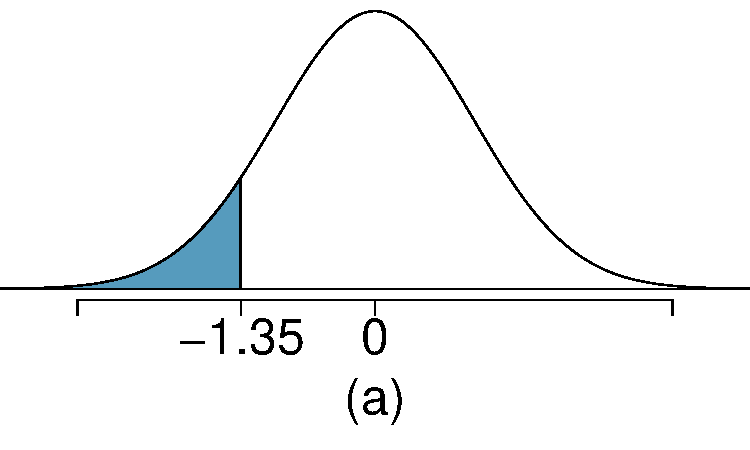
\includegraphics[width=0.23\textwidth]{ch_distributions_oi_biostat/figures/eoce/area_under_curve_1/zltNeg}
	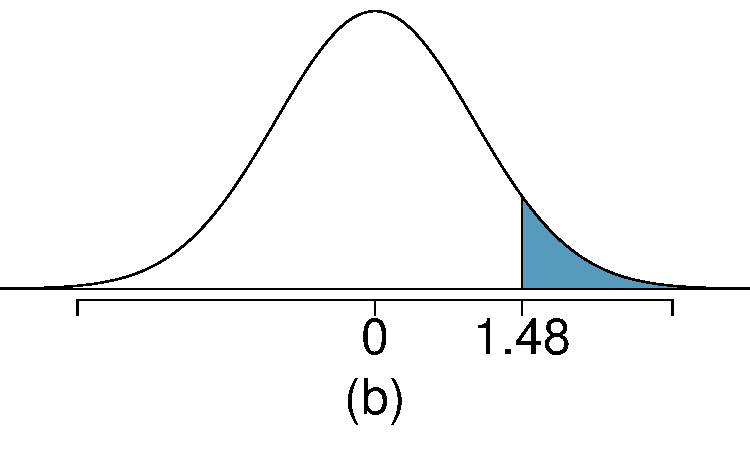
\includegraphics[width=0.23\textwidth]{ch_distributions_oi_biostat/figures/eoce/area_under_curve_1/zgtPos}
	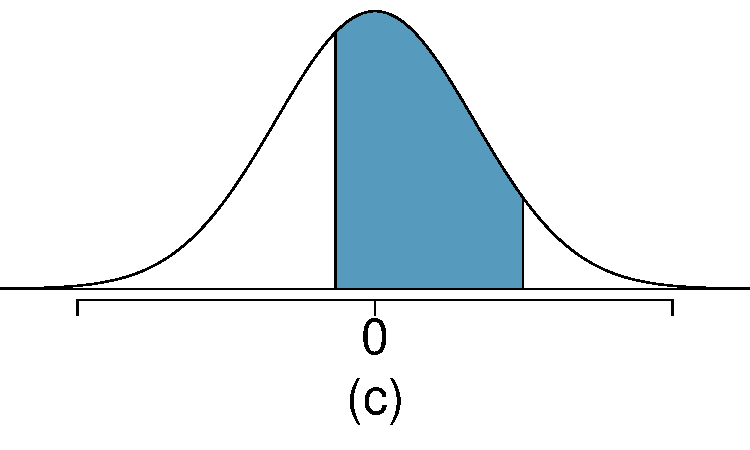
\includegraphics[width=0.23\textwidth]{ch_distributions_oi_biostat/figures/eoce/area_under_curve_1/zBet}
	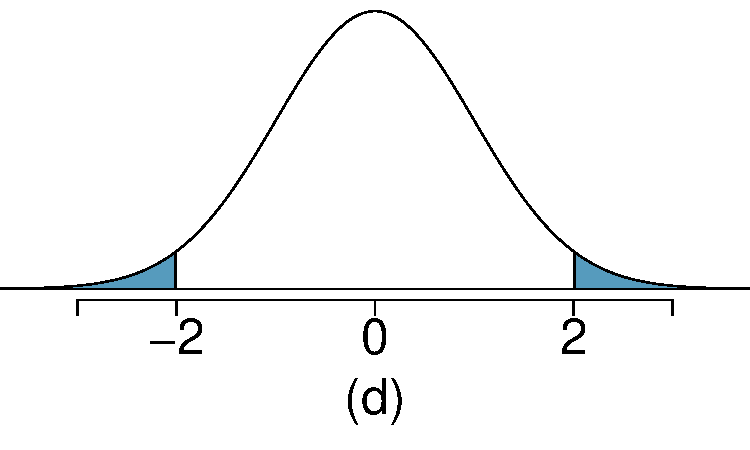
\includegraphics[width=0.23\textwidth]{ch_distributions_oi_biostat/figures/eoce/area_under_curve_1/zgtAbs}}

% 13

\eocesol{(a)~0.005. (b)~0.911. (c)~0.954. (d)~1.036. (e)~-0.842}

% 14

\eocesol{(a)~Verbal: $N(\mu = 151, \sigma = 7)$, Quant: $N(\mu = 153, \sigma = 7.67)$. $Z_{VR} = 1.29$, $Z_{QR} = 0.52$. She did better on the Verbal Reasoning section since her Z-score on that 
	section was higher.\\
	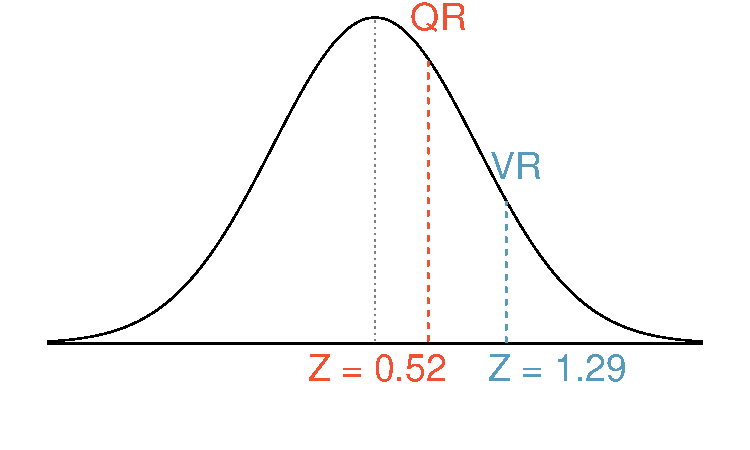
\includegraphics[width=0.3\textwidth]{ch_distributions_oi_biostat/figures/eoce/gre_intro/gre_intro.pdf} \\
	(b)~$Perc_{VR} = 0.9007 \approx 90\%$, $Perc_{QR} = 0.6990 \approx 70\%$. $100\% - 90\% = 10\%$ did better than her on VR, and $100\% - 70\% = 30\%$
	did better than her on QR. \\
	(c)~159.
	(d)~147.}

% 15

\eocesol{(a)~13.8\%. (b)~37.7\%. (c)~3,353 seconds. (d)~6,295 seconds.}

% 16

\eocesol{The tail area lower than -2.5 units on the standard normal curve equals 0.0062. Thus, .62\% of young adults suffer from osteoporosis according to this criterion.}


% 17

\eocesol{(a)~0.115. (b)~The coldest 10\% of days are colder than 70.59\degree F.}


% 18

\eocesol{(a)~0.099. (b)~The largest 5\% of egg clutches have volume of more than 1507.5 mm$^3$. }

% 19

\eocesol{(a)~0.023. (b)~72.66 mg/dL.}

% 20

\eocesol{The middle 95\% of this distribution is defined by 0.260 and 6.140 $\mu$g/dl.}

% 21

\eocesol{(a)~82.4\%. (b)~About 38 years of age.}

% 22

\eocesol{(a)~$\frac{x-\mu}{\sigma} = Z$. $\sigma = 15.58$. (b)~39.04 mg/dL.}

% 23

\eocesol{Let $A$ be the event of scoring above 2100 and $B$ be the event of scoring above 1900. The question asks for $P(A|B)$. By the definition of conditional probability, $P(A|B) = \frac{P(A \textrm{ and } B)}{P(B)}$. In the context of this question, $P(A \textrm{ and } B = P(A)$, since if someone scores above 2100, they necessarily score above 1900. $P(A) = 0.023$, $P(B) = 0.091$. $P(A|B) = 0.249$. }

% 24

\eocesol{(a)~$n = 50$, and $p = 0.70$. $\mu = np = 35$. $\sigma = \sqrt{np(1-p)} = 3.24$. \\
	(b)~Both $np$ and $n(1-p)$ are greater than 10. Thus, it is valid to approximate the distribution as $X \sim N(35, 3.24)$, where $X$ is the number of 18-20 year olds who have consumed alcohol. $P(X \geq 45) = 0.001$. }

% 25

\eocesol{(a)~$n = 120$, and $p = 0.90$.  $\mu = np = 108$. $\sigma = \sqrt{np(1-p) = 3.29}$. \\
	(b)~Both $np$ and $n(1-p)$ are greater than 10. Thus, it is valid to approximate the distribution as $X \sim N(108, 3.29)$, where $X$ is the number of adults who have had chickenpox as a child. $P(X \leq 105) = 0.181$.}

% 26

\eocesol{Let $X$ represent the number of students who accept the the offer; $X \sim \textrm{Bin}(2500, 0.70)$. This distribution can be approximated by a $N(1750, 22.91)$. The approximate probability that the school does not have enough dorm room spots equals $P(X \geq 1,786) = 0.06$.}

% 27

\eocesol{The data appear to follow a normal distribution, since the points closely follow the line on the normal probability plot. There are some small deviations, but this is to be expected for such a small sample size.}


%% 3.4 POISSON DISTRIBUTION

% 28 

\eocesol{(a)~$P(X = 2) = \frac{\exp^{-2}(2^2)}{2!} = 0.271$. (b)~$P(X \leq 2) = P(X = 0) + P(X = 1) + P(X = 2) = 0.677$. (c)~$P(X \geq 3) = 1 - P(X \leq 2) = 0.323$.}

% 29

\eocesol{(a)~$\lambda = 1$; thus $\mu = \lambda = 1$ and $\sigma = \sqrt{\lambda} = 1$. (b)~Let $X$ represent the number of typos made in an hour. $P(X \leq 3) = 0.981$. (c)~Let $Y$ represent the number of typos made in 3 hours; $\lambda = 1$, $t = 3$. $P(Y \geq 5) = 0.185$. }

\textC{
\end{multicols}
\newpage
\begin{multicols}{2}
}

% 30

\eocesol{(a)~$p = \frac{8}{10^6}$, $n = 1.4 \times 10^6$. $\lambda = np = 11.2$ The expected number of cases in a given year is 11.2\\
	(b)~$P(X \geq 15) = 1 - P(X \leq 14) = 0.161$. \\
	(c)~For Brooklyn, $\lambda = 3.6$. The probability of 10 or more cases in Brooklyn in a given year is 0.004. }

% 31 

\eocesol{(a)~$\lambda$ for a population of 2,000,000 male births is 400. The probability of at most 380 newborn males with hemophilia is $P(X \leq 380$), where $X \sim \textrm{Pois}(400)$: 0.165. \\
	(b)~$P(X \geq 450) = 0.0075$. \\
	(c)~The number of male births is (1/2)(1,500,000) = 750,000. The rate $\lambda$ for one year is 150. Over 5 years, the rate $\lambda$ is 750. The expected number of hemophilia births over 5 years is 750 and the standard deviation is $\sqrt{750} = 27.39$.}

% 32

\eocesol{(a)~The number of non-Hispanic whites is $(769,000)(0.73) = 561,370$; $\lambda$ = $(6.8/100,000)(561,370) = 38.17$. $P(X \geq 146) = 2.62 \times 10^{-40}$. \\
	(b)~To compute the observed rate in terms of deaths per 100,000 non-Hispanic whites, divide the number of overdose fatalities reported by the total number of non-Hispanic whites, and multiply by 100,000 $\rightarrow$ $(146,000/561,370)(100,000) = 26.0078$. \\
	(c)~The observed rate $\lambda$ is simply 146, since the population did not change. $P(X \geq 165) = 0.065$.}

%% 3.5 DISTRIBUTIONS RELATED TO BERNOULLI TRIALS

% 33

\eocesol{(a)~On average, 2 women would need to be sampled in order to select a married woman ($\mu = 1/p = 2.123$), with standard deviation 1.544 ($\sigma = \sqrt{\frac{(1-p)}{p^2}}$). \\
	(b) $\mu = 3.33$. $\sigma = 2.79$. \\
	(c)~Decreasing the probability increases both the mean and the standard deviation. }

% 34 
\eocesol{(a)~On average, about 3 donors would need to be sampled before selecting a Type O+ individual ($\mu = 2.70$), with standard deviation 2.15. \\
	(b)~Let $X$ represent the number of donors that must be sampled to find a Type O+ individual; $X \sim \textrm{Geom}(0.37)$. $P(X = 4) = 0.093$. \\
	(c)~$P(X > 4) =  0.158$. \\
	(d)~Let $Y$ represent the number of donors that must be sampled to find a Type O- individual; $Y \sim \textrm{Geom}(0.08)$. $P(X \leq 4) = 0.284$. \\
	(e)~$\mu = 12.5$, $\sigma = 11.99$. \\
	(f)~$P(X \leq 5) = 0.341$.}

% 35

\eocesol{(a)~Let $X$ represent the number of stocks that must be sampled to find an infected stock; $X \sim \textrm{Geom}(0.30)$. $P(X \leq 5) = 0.832$.\\
	(b)~$P(X \leq 6) = 0.882$.\\
	(c)~$P(X \geq 3) = 1 - P(X \leq 2) = 0.49$. }

% 36 

\eocesol{(a)~0.142, negative binomial with $k = 10$, $p = 0.65$.\\
	(b)~0.212, binomial with $n = 15$, $p = 0.65$.\\
	(c)~0.080, geometric with $p = 0.65$. }

% 37 

\eocesol{(a)~0.102, geometric with $p = 1994/14,604 = 0.137$.\\
	(b)~0.259, binomial with $n = 10$, $p = 0.137$.\\
	(c)~0.033, negative binomial with $k = 3$, $p = 0.137$\\
	(d)~The mean and standard deviation of a negative binomial random variable with $k = 4$ and $p = 0.137$ are 29.30 and 13.61, respectively.}

% 38

\eocesol{(a)~0.04, negative binomial with $k = 3$, $p = 0.15$.\\
	(b)~Since the trials are independent, the probability of making the next serve is 0.15.\\
	(c)~The first scenario is a probability statement about 3 successful serves occurring with 10 trials; the second, however, is only asking about the next serve.}

% 39

\eocesol{(a)~$\mu = 2.05$; $\sigma^2 = 1.77$. \\
	(b)~Let $X$ represent the number of soapy-taste detectors; $X \sim \textrm{HGeom}(1994, 14604-1994,15)$. $P(X = 4) = 0.09435$.\\
	(c)~$P(X \leq 2) = 0.663$.\\
	(d)~0.09437, from the binomial distribution. With a large sample size, sampling with replacement is highly unlikely to result in any particular individual being sampled again. In this case, the hypergeometric and binomial distributions will produce equal probabilities.}

% 40

\eocesol{(a)~0.664, binomial with $n = 7$, $p = 0.44$.\\
	(b)~0.246, geometric with $p = 0.44$.\\
	(c)~0.022, hypergeometric with $m = 350-154$, $N-m = 154$, $n = 10$. \\
	(d)~0.030, binomial with $n = 50$, $p = 0.44$.\\}



\textC{}
\end{multicols}
\newpage


%%%%%%%%%%%%%%%%%%%%%%%%%%%%%%%%%%%%%%%%%%%%%%%%%%%%%%%%%%%%%%%%%%%%%%%%%%%%%%%%%%%%%%%%%%%%%%%%%%%%%%%%%%%%%%

%_______________
\eocesolch{Foundations for inference}



%_______________
\begin{multicols}{2}

% 1

\eocesol{(a)~Mean. Each individual reports a numerical value: a number of days where physical health was not good.
(b)~Proportion. Each respondent responds Yes or No, so this is a categorical variable and a proportion is used.
(c)~Proportion. Individuals respond Yes or No if they had exercised, so this is a categorical 
variable and a proportion is used.
(d)~Mean. The response is a numerical number, a distance. 
(e)~Mean. The respondents reported the number of cigarettes smoked a day. It is important to note that this is a conditional average, conditioned on if the person had smoked during the past 30 days.}

% 3

\eocesol{(a)~Mean: 0.7. Median:0.72.
(b)~SD: 0.06. IQR: $0.75-0.67=0.08$.
(c)~$Z_{0.86} = \frac{0.86-0.7}{0.06} = 2.67$. A body size of 0.86 cm is considered unusual since it is beyond 2 SD of the mean. 
$Z_{0.6} =\frac{0.7-0.6}{0.06}= 1.67$, which is not considered unusual. A body size of 0.6cm is within 2 SD of the mean. 
(d)~No the study is not invalidated. There simply exists sampling variation among sample means. The sample that the original researchers observed is likely to be different than the new sample of 129 frogs. These point estimates both approximate the population parameter, but values vary from one sample to another.  
(e)~The standard error measures variability in point estimates like the sample mean. The equation for standard error is $\frac{s}{\sqrt{n}}$.  $0.06/\sqrt{129} =0.005$ is the standard error for this sample mean.}

% 5

\eocesol{(a)The number of observations in a sample is needed to calculate the standard error. The equation for standard error is $\frac{s}{\sqrt{n}}$. 
(b) $\frac{s}{\sqrt{n}} = \frac{5.81}{\sqrt{595}} = 0.24$. 
(c) Yes. The distribution of ages in the sample is skewed right. However, the normality of the sampling distribution of the sample mean depends on the number of observations in the sample size. Because the sample is significantly larger than 30 observations, the sampling distribution is likely to be normal. Assumptions of independence have not yet been verified, but the sampling distribution can be approximated to a normal distribution regardless of skew. 
(e)Yes, $Z=\frac{24.41-24.34}{2.71}=0.03$. The FAMuSS sample mean is extremely close to the average age reported by the Census.}

% 7

\eocesol{(a) No the researchers do not. Imagine remeasuring the 507 individuals in inches and then taking the mean. This process is equivalent to simply converting the mean itself from centimeters to inches. 
(b) The mean in inches is 67.36. The median is 67.05 inches. 
(c) The equation for standard error is $\frac{s}{\sqrt{n}}$. If the number of observation decreases, the standard error will get larger. More data means less variability, and vice versa. 
}

%9
\eocesol{(a) We are 95\% confidence that the number of hours that U.S. residents have to relax or pursue activities that they enjoy is between 3.53 and 3.83 hours. 
(b) 95\% of confidence intervals calculated from independent random samples would contain the true average number of hours that U.S. results have to relax or pursue activities after an average work day. 
(c) They will be less confidence than 95\% that the confidence interval contains the population parameter. Less confidence leads to a narrower confidence interval. 
(d) To guarantee that the population parameter is captured, the interval needs to be $(0, 24)$. This does not provide any insight to the actual number of hours that U.S. residents have to enjoy. \emph{Note:} An answer of $(-\infty, \infty)$ is nonsensical. There can't be $-\infty$ or $\infty$ hours per day. Always remember the context of the question when preforming inference.
}

% 11

\eocesol{(a) Notice that the confidence interval has shifted left by 3 units. Assuming that the confidence level and the standard error has stayed the same, the point estimate is 3 units smaller than the one observed from \data{BRFSS BMI}. 
(b) The center is wholly determined by the point estimate. The width of the confidence interval is determined by the standard error (standard deviation and number of observations in the sample) and the confidence level. 
(c) The sample is already observed so the standard error cannot change. To have a larger width, the confidence level must increase. 
(d) Without changing the confidence level, the width can be modified though its standard error (standard deviation and number of observations). The number of observations can increase so that the standard error is smaller. A confidence interval with a smaller standard error will have a narrower width.
}

% 13

\eocesol{(a)~False. Provided the data distribution is not very strongly skewed ($n = 64$ in 
this sample, so we can be slightly lenient with the skew), the sample mean will 
be nearly normal, allowing for the method normal approximation described.
(b)~False. Inference is made on the population parameter, not the point 
estimate. The point estimate is always in the confidence interval.
(c)~True.
(d)~False. The confidence interval is not about a sample mean.
(e)~False. To be more confident that we capture the parameter, we need a wider 
interval. Think about needing a bigger net to be more sure of catching a fish in 
a murky lake.
(f)~True. Optional explanation: This is true since the normal model was used to 
model the sample mean. The margin of error is half the width of the interval, 
and the sample mean is the midpoint of the interval.
(g)~False. In the calculation of the standard error, we divide the standard 
deviation by the square root of the sample size. To cut the SE (or margin of 
error) in half, we would need to sample $2^2 = 4$ times the number of people in 
the initial sample.}



% 15

\eocesol{Independence: We do not know that the sample is less than 10\% of the population or that is independent. Size: the sample size is greater than 30. Skew: The data is skewed if students investigate the data itself. However the sample size is so larger than the skewness will have little effect on the normality of the sample mean. The independence assumption is fairly suspect but a confidence interval is calculated. 95\% CI: $(26.7 \pm 1.96 \times \frac{25.93}{222}) \rightarrow (23.29, 30.11)$. We are 95\% confident that the infant morality rate of the world lies between 23.29 and 30.11. Assuming that we have a null hypothesis: $\mu = 32$, evidence from the confidence interval rejects it. An infant morality rate of 32 is not included in the confidence interval. The evidence from the CIA disagrees with the WHO estimate. }




% 17
\eocesol{The sample mean is the center of the confidence interval. The margin of error is the half-width of the confidence interval. The sample standard deviation is calculated from the margin of error: $\textrm{margin} = 1.65 * \frac{s}{\sqrt{n}}$. $\bar{x} = 71$, $\mathrm{margin of error} = 6$, and $s = 36$. }


% 19

\eocesol{(a) True. A 95\% confidence interval lies within a 99\% confidence interval. The 99\% confidence interval is wider. 
(b) False. A 95\% does not completely contain a 90\% confidence interval. Consider the boundary values of a 95\% confidence interval. These are not within a 90\% confidence interval. 
(c) False. $\alpha$ is also the probability of making a Type 1 Error. Decreasing $\alpha$ decreases the probability of making a Type 1 Error. 
(d) False. The population parameter is 5 at a certain confidence interval, or a Type 2 Error could have been committed.
(e) False. Rejecting the null hypothesis gives evidence that the alternative is true, $\mu > 5$. 
(f) False. Rejecting the null hypothesis gives evidence that the alternative is true but not for a specific value like 7. 
(g) False. $\alpha = 0.05$ is a value that is traditionally chosen, but $\alpha$ can be ideal depending on the varying contexts and implications of the hypothesis test. 
}

% 21

\eocesol{(a) $H_0:$ There is no difference between the IQ levels of mothers and fathers of gifted children ($\mu_\mathrm{mothers} = \mu_\mathrm{fathers}$). $H_A$: There exists a difference between the IQ levels of mothers and fathers of gifted children ($\mu_\mathrm{mothers} \neq \mu_\mathrm{fathers}$). 
(b) $H_0$: The average infant morality rate in the world is 32 ($\mu = 32$). $H_A$: The average infant morality rate in the world is not 32 ($\mu \neq 32$). 
(c) $H_0$: There is no noticeable difference between the MCAT scores of 2014 and in 2004 ($\mu_{2014} = \mu_{2004}$. $H_A$: There is a difference between the average 2014 MCAT score and the average 2004 MCAT score ($\mu_{2014} \neq \mu_{2004}$). 
}

%23

\eocesol{(a) The hypotheses are listed in Section~\ref{hypothesisFramework}. Let $\alpha = 0.05$. The T-statistic is $\frac{26.53-25.3}{5.84/\sqrt{40}} = 1.33$. Use \textsf{R} to find the p-value (\textsf{2*(1-pnorm(1.33))}=0.18). The p-value is greater than $\alpha$. We do not have sufficient evidence to reject the null hypothesis. We are 95\% confident that the average adult population in the U.S. has an equivalent BMI to U.S. adults 20 years ago.
(b) The confidence interval created in Section~\ref{calculate95confidence} included 25.3. The conclusions from the confidence interval and the hypothesis testing both agree with each other.}



%25
\eocesol{The hypotheses should be about the population mean ($\mu$), not the sample mean($\overline{x}$). The sample mean is already known, and no hypothesis test is needed for information about the sample mean.
Correction: 
\begin{align*}
H_0&: \mu = 100\\
H_A&: \mu > 100
\end{align*}}

% 27

\eocesol{(a)~This claim does is not supported since 3 hours (180 minutes) is not in 
the interval.
(b)~2.2~hours (132 minutes) is in the 95\% confidence interval, so we do not 
have evidence to say she is wrong. However, it would be more appropriate to use 
the point estimate of the sample.
(c)~A 99\% confidence interval will be wider than a 95\% confidence interval, 
meaning it would enclose this smaller interval. This means 132 minutes would be 
in the wider interval, and we would not reject her claim based on a 99\% 
confidence level.}


% 29

\eocesol{(a)~Independence: The sample is random and 64 patients would almost certainly 
make up less than 10\% of the ER residents. The sample size is at least 30. No 
information is provided about the skew. In practice, we would ask to see the 
data to check this condition, but here we will make the assumption that the skew 
is not very strong.
(b)~$H_0: \mu = 127$. $H_A: \mu \neq 127$. $Z=2.15$ $\to$ p-value $= 0.0316$. 
Since the p-value is less than $\alpha=0.05$, we reject $H_0$. The data provide 
convincing evidence that the average ER wait time is different from last year and perhaps has increased over the last year.
(c)~Yes, it would change. The p-value is greater than 0.01, meaning we would 
fail to reject $H_0$ at $\alpha = 0.01$.}


% 31

\eocesol{$H_0: \mu = 130$. $H_A: \mu \ne 130$. $Z=1.39$ $\to$ p-value $= 0.1646$, which 
is larger than $\alpha=0.05$. The data do not provide convincing evidence that 
the true average calorie content in bags of potato chips is different than 130 
calories.}

%33
\eocesol{The alternative hypothesis is one sided so the T-statistic is 1.65. $T = \frac{\bar{x}-34}{10/\sqrt{65}}\rightarrow \bar{x} = 36.04$}


%35
\eocesol{(a)~$H_0$: Anti-depressants do not help symptoms of Fibromyalgia. $H_A$: Anti-
depressants do treat symptoms of Fibromyalgia. Remark: Diana might also have 
taken special note if her symptoms got much worse, so a more scientific approach 
would have been to use a two-sided test. If you proposed a two-sided 
approach, your answers in~(b) and~(c) will be different.
(b)~Concluding that anti-depressants work for the treatment of Fibromyalgia 
symptoms when they actually do not.
(c)~Concluding that anti-depressants do not work for the treatment of 
Fibromyalgia symptoms when they actually do.
(d) If she makes a Type 1 error, she will continue taking medication that does not actually read her disorder. If she makes a Type 2 error, she will stop taking medication that could treat her disorder.}

% 37
\eocesol{(a) If the null hypothesis is rejected incorrectly, the regulators concluded that the adverse effect was higher in those taking the drug than those who did not take the drug when in fact, the rates were the same for the two groups. 
(b) If the null hypothesis is not rejected but should have been, the regulators failed to identify that the adverse effect was higher in those taking the drug. 
(c) Answers may vary slightly. If all 403 drugs last year are alright, then about $403 \times 0.05 \approx 20$ drugs would have a Type 1 error. Of the 42 suspect drugs, we would expect about $20/42$ of the drugs to represent an error and $22/42\approx 52\%$ to represent drugs with adverse effects. 
(d) There is not enough information to tell. 
}

% 39
\eocesol{Because the sample size is 20, use the $t$-distribution instead. The sample mean is still the midpoint of the confidence interval. The margin of error is still the half-width of the confidence interval. The sample standard deviation is calculated form the margin of error and the standard error. The sample standard deviation is the only answer different from Exercise~\ref{backwardspt1}. It is $s=\mathrm{margin of error}/1.729 \times \sqrt{20} = 15.52$.The sample standard deviation is must smaller than in Exercise~\ref{backwardspt1}. 
}

% 41
\eocesol{(a) $df = 6-1 = 5, t_5^{\star}=2.02$ (column with two tails of 0.10, row with $df = 5$).
(b) $df = 21-1 = 20, t_{20}^{\star}=2.53$ (column with two tails of 0.02, row with $df = 20$)  
(c) $df = 29-1 = 28, t_{28}^{\star}=2.05$
(d) $df = 11, t_{11}^{\star}=3.11$}

% 43
\eocesol{The alternative hypothesis is two-sided so the T-statistic must equal 2.09 because the sample size is less than 30 \textsf{qt(1.975, 19)}. $T = \frac{\bar{x}-60}{8/\sqrt{20}}\rightarrow \bar{x} = 63.74$. }


% 45
\eocesol{(b) The distribution is unimodal and extremely right skewed. . The mean is 1.17\%, and the median is 0.5\%, confirming the skewness. The standard deviation is 2.51\% and has apparent outliers toward the higher percent values. 
(c) The sampling distribution for size 5 is extremely skewed still but as the sample size gets larger, the sampling distribution becomes more normal. As the sample size increases, the sampling distribution gets more unimodal, symmetric with variability decreasing. At sample size $n=100$, the sampling distribution appears extremely normal. This is consist with the Central Limit Theorem. Sharp students will question why the sampling distribution for $n=5$ appears to be the opposite skew, left skewed, of the population distribution. These students should have a closer look into the data and observe that the skewness of the population distribution causes the extreme drop. The skewness causes the sampling distribution to appear left skewed.}

% 47
\eocesol{The standard deviation is 2.51. For all 3 sampling distributions, the mean is the population mean, 1.16\%. The standard deviation for each sampling distribution is $\frac{2.51}{\sqrt{n}}$. $SE_5 = 1.12$, $SE_{30} = 0.46$, and $SE_{100} = 0.25$. The distributions in Exercise~\ref{countiespt1} agree with the values. As the sample size increases, the standard errors decrease. The sampling variation in the graphs also decreases.}

% 49
\eocesol{The centers are the same in each plot, and each data set is from a nearly normal 
distribution, though the histograms may not look very normal since each 
represents only 100 data points. The only way to tell which plot corresponds to 
which scenario is to examine the variability of each distribution. Plot B is the 
most variable, followed by Plot A, then Plot C. This means Plot B will 
correspond to the original data, Plot A to the sample means with size 5, and 
Plot C to the sample means with size 25.}

% 51
\eocesol{(a) The distribution is left skewed. 
(b) Most counties would have more than 82.89\% of their population to be White.
(c) Sheboygan County is an individual observation. We cannot estimate a probability for a single county.
(d) Even through the population distribution is not normal, the conditions for inference are reasonably satisfied, with the possible exception of skew. If the skew isn't very strong (check the data to see), the Central Limit Theorem can be used to estimate this probability. Use $\mathcal{N}(82.89, 16.85/\sqrt{30}: Z = \frac{99-82.89}{16.85/\sqrt{30}} = 5.24 \rightarrow$ p-value $\approx 0$. 
(e) The standard error of the mean would decrease by a factor of $\sqrt{2}$. 
(f) With the same reasoning as (d): Use $\mathcal{N}(82.89, 16.85/\sqrt{60}: Z = \frac{99-82.89}{16.85/\sqrt{60}} = 7.41 \rightarrow$ p-value $\approx 0$. 
(g) Answers may vary but the the theorem applies to this problem in general, with one main caveat. A normal distribution has support from $(-\infty,\infty)$. With most applications, this is not an issue. However, with a mean of 82.89\% and such a large standard deviation, values within the first standard deviation are almost larger than 100\%. In this exercise, these values are nonsensical. 
 }


% 53

\eocesol{(a) $H_0: \overline{\mathrm{weight}_{\mathrm{smoke}}} =\overline{\mathrm{weight}_{\mathrm{nonsmoker}}}$ and $H_A: \overline{\mathrm{weight}_{\mathrm{smoke}}} \neq\overline{\mathrm{weight}_{\mathrm{nonsmoker}}}$. The point estimate is the difference in means of the 50 babies who had a mother who smoked and the mean of the 50 babies who had a mother who did not smoke. In \textsf{R}, the point estimate is  $\overline{\mathrm{weight}_{\mathrm{smoke}}} -\overline{\mathrm{weight}_{\mathrm{nonsmoker}}} = 6.78 - 7.18 = -0.4$. 
(b) North Carolina observed a p-value that is less than their $\alpha$ value. Therefore they cannot reject the null hypothesis and conclude that the weight of babies is not different between mothers who smoke and those who do not smoke. 
(c) Yes. A confidence interval of differences should contain 0 if North Carolina concluded that there was no statistically significant difference in the mean weights between these two populations.}


% 55

\eocesol{(a) $H_0: p_{\mathrm{smoke}} =p_{\mathrm{nonsmoker}}$ and $H_A: p_{\mathrm{smoke}} > p_{\mathrm{nonsmoker}}$. 
(b) North Carolina observed a p-value that is greater than their $\alpha$ value. Therefore they can reject the null hypothesis and conclude that there was a higher percent of babies who were born prematurely from mothers who smoked than from mothers who did not smoke. 
(c) No. A hypothesis test concluding that there is an observed difference should not include 0, which indicates that there is no observed difference. Because the alternative hypothesis is one-sided, the difference between the two population means if the difference were defined as smoker - nonsmoker would be positive.}

% 57
\eocesol{(a) $H_0: \overline{x}_\mathrm{female} = \overline{x}_\mathrm{male}$. $H_A: \overline{x}_\mathrm{female} \neq \overline{x}_\mathrm{male}$.
(b) Define the point estimate as $\bar{x}_\mathrm{female} - \bar{x}_\mathrm{male} = 1.40$ cm. $H_0: \bar{x} = 0$. $H_A: \bar{x} \neq 0$ if $\bar{x} = \bar{x}_\mathrm{female}-\bar{x}_\mathrm{male}$. 
(c) $T = \frac{1.4-0}{0.85} = 1.65$
(d) This is a two sided alternative test so the p-value is, in \textsf{R}, \textsf{2*(1-pnorm(1.65))} = 0.1. We also know that 1.65 is the critical value for 90\% in a normal distribution. 
(e) Because the p-value is larger than $\alpha = 0.05$, we cannot reject the null hypothesis. We conclude that there is no statistically significant difference in total body length at the 95\% confidence level between male and female possums.}

%59

\eocesol{(a)~Scenario I is higher. Recall that a sample mean based on less data tends to 
be less accurate and have larger standard errors.
(b)~Scenario I is higher. The higher the confidence level, the higher the 
corresponding margin of error.
(c)~They are equal. The sample size does not affect the calculation of the p-
value for a given Z-score.
(d)~Scenario I is higher. If the null hypothesis is harder to reject 
(lower $\alpha$), then we are more likely to make a Type~2 Error when the 
alternative hypothesis is true.}

% 61

\eocesol{(a) The researchers assume that the standard deviation of the previous sample serves as an estimate for the population standard deviation.  $0.5\geq 1.96 \times SE \rightarrow 0.5\geq 1.96 \times \frac{2.57}{\sqrt{n}} \rightarrow \sqrt{n} \geq 10.07 \rightarrow n\geq 101.49$. The sample should be 102 possums. 
(b) Similarly $0.5\geq 2.58 \times SE \rightarrow 0.5\geq 2.58 \times \frac{2.57}{\sqrt{n}} \rightarrow \sqrt{n} \geq 13.26 \rightarrow n\geq 175.86$. The sample should be 176 possums. The number of possums is much higher than in part(a). This should confirm students intuitions. 
}

% 61

\eocesol{(a) The null hypothesis would be that the mean this year is also 128 minutes. The alternative hypothesis would be that the mean is different from 128 minutes. 
(b) First calculate the SE: $\frac{39}{\sqrt{64}} = 4.875$. Next, identify the Z scores that would reject in rejecting $H_0: Z_\mathrm{lower} = -1.96, Z_\mathrm{upper} = 1.96$. In each case, calculate the corresponding sample mean cutoff: $\bar{x}_\mathrm{lower} = 118.445$ and $\bar{x}_\mathrm{upper} = 137.555$. 
(c) Construct Z scores for the values from part (b) but using the supposed true distribution (i.e. $\mu = 135$), i.e. not using the null value ($\mu = 128$). The probability of correctly rejecting the null hypothesis would be $0.003 + 0.3015 = 0.3018$ using these two cutoffs, and the probably of a Type 2 error would then be $1-0.3018 = 0.6982$. }



\end{multicols}



%%%%%%%%%%%%%%%%%%%%%%%%%%%%%%%%%%%%%%%%%%%%%%%%%%%%%%%%%%%%%%%%%%%%%%%%%%%%%%%%%%%%%%%%%%%%%%%%%%%%%%%%%%%%%%
\begin{comment}




\eocesolch{Inference for numerical data}


\begin{multicols}{2}

% 1
\eocesol{(a)~$df=6-1=5$, $t_{5}^{\star} = 2.02$ (column with two tails of 0.10, row with $df=5$).
(b)~$df=21-1=20$, $t_{20}^{\star} = 2.53$ (column with two tails of 0.02, row with $df=20$).
(c)~$df=28$, $t_{28}^{\star} = 2.05$.
(d)~$df=11$, $t_{11}^{\star} = 3.11$.}

% 3
\eocesol{(a)~between 0.025 and 0.05
(b)~less than 0.005
(c)~greater than 0.2
(d)~between 0.01 and 0.025}

% 5
\eocesol{The mean is the midpoint: $\bar{x} = 20$. Identify the margin of error: $ME = 1.015$, then use $t^{\star}_{35} = 2.03$ and $SE=s/\sqrt{n}$ in the formula for margin of error to identify $s = 3$.}

% 7
\eocesol{(a)~$H_0$: $\mu = 8$ (New Yorkers sleep 8 hrs per night on average.) $H_A$: $\mu < 8$ (New Yorkers sleep less than 8 hrs per night on average.)
(b)~Independence: The sample is random and from less than 10\% of New Yorkers. The sample is small, so we will use a $t$-distribution. For this size sample, slight skew is acceptable, and the min/max suggest there is not much skew in the data. $T = -1.75$. $df=25-1=24$.
(c)~$0.025 <$ p-value $<0.05$. If in fact the true population mean of the amount New Yorkers sleep per night was 8 hours, the probability of getting a random sample of 25 New Yorkers where the average amount of sleep is 7.73 hrs per night or less is between 0.025 and 0.05.
(d)~Since p-value $<$ 0.05, reject $H_0$. The data provide strong evidence that New Yorkers sleep less than 8 hours per night on average.
(e)~No, as we rejected $H_0$.}

% 9
\eocesol{$t^{\star}_{19}$ is 1.73 for a one-tail. We want the lower tail, so set -1.73 equal to the T-score, then solve for $\bar{x}$: 56.91.}


\textC{
\end{multicols}
\newpage
\begin{multicols}{2}
}


% 11
\eocesol{(a)~We will conduct a 1-sample $t$-test. $H_0$: $\mu = 5$. $H_A$: $\mu < 5$. We'll use $\alpha = 0.05$. This is a random sample, so the observations are independent. To proceed, we assume the distribution of years of piano lessons is approximately normal. $SE = 2.2 / \sqrt{20} = 0.4919$. The test statistic is $T = (4.6 - 5) / SE = -0.81$. $df = 20 - 1 = 19$. The one-tail p-value is about 0.21, which is bigger than $\alpha = 0.05$, so we do not reject $H_0$. That is, we do not have sufficiently strong evidence to reject Georgianna's claim. \\
(b)~Using $SE = 0.4919$ and $t_{df = 19}^{\star} = 2.093$, the confidence interval is (3.57, 5.63). We are 95\% confident that the average number of years a child takes piano lessons in this city is 3.57 to 5.63 years. \\
(c)~They agree, since we did not reject the null hypothesis and the null value of 5 was in the $t$-interval.}

% 13
\eocesol{If the sample is large, then the margin of error will be about $1.96 \times 100 / \sqrt{n}$. We want this value to be less than 10, which leads to $n \geq 384.16$, meaning we need a sample size of at least 385 (round up for sample size calculations!).}

% 15
\eocesol{(a)~Two-sided, we are evaluating a difference, not in a particular direction.
(b)~Paired, data are recorded in the same cities at two different time points. The temperature in a city at one point is not independent of the temperature in the same city at another time point.
(c)~$t$-test, sample is small and population standard deviation is unknown.
}

% 17
\eocesol{(a)~Since it's the same students at the beginning and the end of the semester, there is a pairing between the datasets, for a given student their beginning and end of semester grades are dependent.
(b)~Since the subjects were sampled randomly, each observation in the men's group does not have a special correspondence with exactly one observation in the other (women's) group.
(c)~Since it's the same subjects at the beginning and the end of the study, there is a pairing between the datasets, for a subject student their beginning and end of semester artery thickness are dependent.
(d)~Since it's the same subjects at the beginning and the end of the study, there is a pairing between the datasets, for a subject student their beginning and end of semester weights are dependent.}

% 19
\eocesol{(a)~For each observation in one data set, there is exactly one specially-corresponding observation in the other data set for the same geographic location. The data are paired.
(b)~$H_0: \mu_{diff} = 0$ (There is no difference in average daily high temperature between January 1, 1968 and January 1, 2008 in the continental US.) $H_A: \mu_{diff} > 0$ (Average daily high temperature in January 1, 1968 was lower than average daily high temperature in January, 2008 in the continental US.) If you chose a two-sided test, that would also be acceptable. If this is the case, note that your p-value will be a little bigger than what is reported here in part~(d).
(c)~Independence: locations are random and represent less than 10\% of all possible locations in the US. The sample size is at least 30. We are not given the distribution to check the skew. In practice, we would ask to see the data to check this condition, but here we will move forward under the assumption that it is not strongly skewed.
(d)~$Z=1.60$ $\to$ p-value $=0.0548$.
(e)~Since the p-value $> \alpha$ (since not given use 0.05), fail to reject $H_0$. The data do not provide strong evidence of temperature warming in the continental US. However it should be noted that the p-value is very close to 0.05.
(f)~Type~2 Error, since we may have incorrectly failed to reject $H_0$. There may be an increase, but we were unable to detect it.
(g)~Yes, since we failed to reject $H_0$, which had a null value of 0.}

% 21
\eocesol{(a)~(-0.03, 2.23).
(b)~We are 90\% confident that the average daily high on January 1, 2008 in the continental US was 0.03 degrees lower to 2.23 degrees higher than the average daily high on January 1, 1968.
(c)~No, since 0 is included in the interval.}


\textC{
\end{multicols}
\newpage
\begin{multicols}{2}
}


% 23
\eocesol{(a)~Each of the 36 mothers is related to exactly one of the 36 fathers (and vice-versa), so there is a special correspondence between the mothers and fathers.
(b)~$H_0: \mu_{diff} = 0$. $H_A: \mu_{diff} \ne 0$. Independence: random sample from less than 10\% of population. Sample size of at least 30. The skew of the differences is, at worst, slight. $Z = 2.72$ $\to$ p-value $= 0.0066$. Since p-value $<$ 0.05, reject $H_0$. The data provide strong evidence that the average IQ scores of mothers and fathers of gifted children are different, and the data indicate that mothers' scores are higher than fathers' scores for the parents of gifted children.}

% 25
\eocesol{No, he should not move forward with the test since the distributions of total personal income are very strongly skewed. When sample sizes are large, we can be a bit lenient with skew. However, such strong skew observed in this exercise would require somewhat large sample sizes, somewhat higher than~30.}

% 27
\eocesol{(a)~These data are paired. For example, the Friday the 13th in say, September 1991, would probably be more similar to the Friday the 6th in September 1991 than to Friday the 6th in another month or year.
(b)~Let $\mu_{diff} = \mu_{sixth} - \mu_{thirteenth}$. $H_0: \mu_{diff} = 0$. $H_A: \mu_{diff} \ne 0$.
(c)~Independence: The months selected are not random. However, if we think these dates are roughly equivalent to a simple random sample of all such Friday 6th/13th date pairs, then independence is reasonable. To proceed, we must make this strong assumption, though we should note this assumption in any reported results. With fewer than 10 observations, we would need to use the $t$-distribution to model the sample mean. The normal probability plot of the differences shows an approximately straight line. There isn't a clear reason why this distribution would be skewed, and since the normal quantile plot looks reasonable, we can mark this condition as reasonably satisfied.
(d)~$T = 4.94$ for $df=10-1=9$ $\to$ p-value $<0.01$.
(e)~Since p-value $<$ 0.05, reject $H_0$. The data provide strong evidence that the average number of cars at the intersection is higher on Friday the 6$^{\text{th}}$ than on Friday the 13$^{\text{th}}$. (We might believe this intersection is representative of all roads, i.e. there is higher traffic on Friday the 6$^{\text{th}}$ relative to Friday the 13$^{\text{th}}$. However, we should be cautious of the required assumption for such a generalization.)
(f)~If the average number of cars passing the intersection actually was the same on Friday the 6$^{\text{th}}$ and $13^{th}$, then the probability that we would observe a test statistic so far from zero is less than 0.01.
(g)~We might have made a Type~1 Error, i.e. incorrectly rejected the null hypothesis.}

% 29
\eocesol{(a)~$H_0: \mu_{diff} = 0$. $H_A: \mu_{diff} \ne 0$. $T=-2.71$. $df=5$. $0.02<$ p-value $<0.05$. Since p-value $<$ 0.05, reject $H_0$. The data provide strong evidence that the average number of traffic accident related emergency room admissions are different between Friday the 6$^{\text{th}}$ and Friday the 13$^{\text{th}}$. Furthermore, the data indicate that the direction of that difference is that accidents are lower on Friday the $6^{th}$ relative to Friday the 13$^{\text{th}}$.
(b)~(-6.49, -0.17).
(c)~This is an observational study, not an experiment, so we cannot so easily infer a causal intervention implied by this statement. It is true that there is a difference. However, for example, this does not mean that a responsible adult going out on Friday the $13^{th}$ has a higher chance of harm than on any other night.}

% 31
\eocesol{(a)~Chicken fed linseed weighed an average of 218.75 grams while those fed horsebean weighed an average of 160.20 grams. Both distributions are relatively symmetric with no apparent outliers. There is more variability in the weights of chicken fed linseed.
(b)~$H_0: \mu_{ls} = \mu_{hb}$. $H_A: \mu_{ls} \ne \mu_{hb}$. We leave the conditions to you to consider. $T=3.02$, $df = min(11, 9) = 9$ $\to$ $0.01<$ p-value $<0.02$. Since p-value $<$ 0.05, reject $H_0$. The data provide strong evidence that there is a significant difference between the average weights of chickens that were fed linseed and horsebean.
(c)~Type~1 Error, since we rejected $H_0$.
(d)~Yes, since p-value $>$ 0.01, we would have failed to reject~$H_0$.}

% 33
\eocesol{$H_0: \mu_C = \mu_S$. $H_A: \mu_C \ne \mu_S$. $T = 3.27$, $df=11$ $\to$ p-value $<0.01$. Since p-value $< 0.05$, reject $H_0$. The data provide strong evidence that the average weight of chickens that were fed casein is different than the average weight of chickens that were fed soybean (with weights from casein being higher). Since this is a randomized experiment, the observed difference can be attributed to the diet.}


\textC{
\end{multicols}
\newpage
\begin{multicols}{2}
}


% 35
\eocesol{$H_0: \mu_{T} = \mu_{C}$. $H_A: \mu_{T} \ne \mu_{C}$. $T=2.24$, $df=21$ $\to$ $0.02<$ p-value $<0.05$. Since p-value $<$ 0.05, reject $H_0$. The data provide strong evidence that the average food consumption by the patients in the treatment and control groups are different. Furthermore, the data indicate patients in the distracted eating (treatment) group consume more food than patients in the control group.}

% 37
\eocesol{Let $\mu_{diff} = \mu_{pre} - \mu_{post}$. $H_0: \mu_{diff} = 0$: Treatment has no effect. $H_A: \mu_{diff} > 0$: Treatment is effective in reducing P.D.T. scores, the average pre-treatment score is higher than the average post-treatment score. Note that the reported values are pre minus post, so we are looking for a positive difference, which would correspond to a reduction in the P.D.T. score. Conditions are checked as follows. Independence: The subjects are randomly assigned to treatments, so the patients in each group are independent. All three sample sizes are smaller than 30, so we use $t$-tests. Distributions of differences are somewhat skewed. The sample sizes are small, so we cannot reliably relax this assumption. (We will proceed, but we would not report the results of this specific analysis, at least for treatment group 1.) For all three groups: $df=13$. $T_1= 1.89$ ($0.025<$ p-value $<0.05$), $T_2=1.35$ (p-value = 0.10), $T_3 = -1.40$ (p-value $>0.10$). The only significant test reduction is found in Treatment 1, however, we had earlier noted that this result might not be reliable due to the skew in the distribution. Note that the calculation of the p-value for Treatment 3 was unnecessary: the sample mean indicated a increase in P.D.T. scores under this treatment (as opposed to a decrease, which was the result of interest). That is, we could tell without formally completing the hypothesis test that the p-value would be large for this treatment group.}

% 39
\eocesol{Difference we care about: 40. Single tail of 90\%: $1.28 \times SE$. Rejection region bounds: $\pm 1.96 \times SE$ (if 5\% significance level). Setting $3.24 \times SE = 40$, subbing in $SE = \sqrt{\frac{94^2}{n} + \frac{94^2}{n}}$, and solving for the sample size $n$ gives 116 plots of land for each fertilizer.}

% 41

\eocesol{Alternative.}

% 43

\eocesol{$H_0$: $\mu_1 = \mu_2 = \cdots = \mu_6$. $H_A$: The average weight varies across some (or all) groups. Independence: Chicks are randomly assigned to feed types (presumably kept separate from one another), therefore independence of observations is reasonable. Approx. normal: the distributions of weights within each feed type appear to be fairly symmetric. Constant variance: Based on the side-by-side box plots, the constant variance assumption appears to be reasonable. There are differences in the actual computed standard deviations, but these might be due to chance as these are quite small samples. $F_{5,65} = 15.36$ and the p-value is approximately 0. With such a small p-value, we reject $H_0$. The data provide convincing evidence that the average weight of chicks varies across some (or all) feed supplement groups.}

% 45
\eocesol{(a)~$H_0$: The population mean of MET for each group is equal to the others. $H_A$: At least one pair of means is different.
(b)~Independence: We don't have any information on how the data were collected, so we cannot assess independence. To proceed, we must assume the subjects in each group are independent. In practice, we would inquire for more details. Approx. normal: The data are bound below by zero and the standard deviations are larger than the means, indicating very strong skew. However, since the sample sizes are extremely large, even extreme skew is acceptable. Constant variance: This condition is sufficiently met, as the standard deviations are reasonably consistent across groups.
(c)~See below, with the last column omitted:\\[-2mm]
\begin{adjustwidth}{-4em}{-4em}
{\tiny
\begin{center}
\renewcommand{\arraystretch}{1.25}
\begin{tabular}{lrrrr}
  \hline
            & Df    & Sum Sq        & Mean Sq   & F value \\ 
  \hline
coffee      & {\textcolor{oiB}{{\scriptsize 4}}}     & {\textcolor{oiB}{{\scriptsize 10508}}}       & {\textcolor{oiB}{{\scriptsize 2627}}}             & {\textcolor{oiB}{{\scriptsize 5.2}}} \\ 
Residuals       & {\textcolor{oiB}{{\scriptsize 50734}}} & 25564819     & {\textcolor{oiB}{{\scriptsize  504}}}         &  \\ 
   \hline
Total           & {\textcolor{oiB}{{\scriptsize 50738}}} & 25575327 \\
\hline
\end{tabular}
\end{center}
}
\end{adjustwidth} \vspace{1mm}
(d)~Since p-value is very small, reject $H_0$. The data provide convincing evidence that the average MET differs between at least one pair of groups.}


\textC{
\end{multicols}
\newpage
\begin{multicols}{2}
}


% 47
\eocesol{(a)~$H_0$: Average GPA is the same for all majors. $H_A$: At least one pair of means are different.
(b)~Since p-value $>$ 0.05, fail to reject $H_0$. The data do not provide convincing evidence of a difference between the average GPAs across three groups of majors.
(c)~The total degrees of freedom is $195 + 2 = 197$, so the sample size is $197+1=198$.}

% 49
\eocesol{(a)~False. As the number of groups increases, so does the number of comparisons and hence the modified significance level decreases.
(b)~True.
(c)~True.
(d)~False. We need observations to be independent regardless of sample size.}

% 51
\eocesol{(a)~$H_0$: Average score difference is the same for all treatments. $H_A$: At least one pair of means are different.
(b)~We should check conditions. If we look back to the earlier exercise, we will see that the patients were randomized, so independence is satisfied. There are some minor concerns about skew, especially with the third group, though this may be acceptable. The standard deviations across the groups are reasonably similar. Since the p-value is less than 0.05, reject $H_0$. The data provide convincing evidence of a difference between the average reduction in score among treatments.
(c)~We determined that at least two means are different in part (b), so we now conduct $K=3\times2/2=3$ pairwise $t$-tests that each use $\alpha=0.05/3 = 0.0167$ for a significance level. Use the following hypotheses for each pairwise test. $H_0$: The two means are equal. $H_A$: The two means are different. The sample sizes are equal and we use the pooled SD, so we can compute $SE=3.7$ with the pooled $df=39$. The p-value only for Trmt 1 vs. Trmt 3 may be statistically significant: $0.01<$ p-value $<0.02$. Since we cannot tell, we should use a computer to get the p-value, 0.015, which is statistically significant for the adjusted significance level. That is, we have identified Treatment 1 and Treatment 3 as having different effects. Checking the other two comparisons, the differences are not statistically significant.}

\end{multicols}

%%%%%%%%%%%%%%%%%%%%%%%%%%%%%




% Chp 6
\eocesolch{Inference for categorical data}

%%%%%%%%%%%%%%%%%%%%%%%%%%%%%

\begin{multicols}{2}

% 1
\eocesol{(a)~False. Doesn't satisfy success-failure condition.
(b)~True. The success-failure condition is not satisfied. In most samples we would expect $\hat{p}$ to be close to 0.08, the true population proportion. While $\hat{p}$ can be much above 0.08, it is bound below by 0, suggesting it would take on a right skewed shape. Plotting the sampling distribution would confirm this suspicion.
(c)~False. $SE_{\hat{p}} = 0.0243$, and $\hat{p} = 0.12$ is only $\frac{0.12 - 0.08}{0.0243} = 1.65$ SEs away from the mean, which would not be considered unusual.
(d)~True. $\hat{p}=0.12$ is 2.32 standard errors away from the mean, which is often considered unusual.
(e)~False. Decreases the SE by a factor of $1/\sqrt{2}$.}

% 3
\eocesol{(a)~True. See the reasoning of 6.1(b).
(b)~True. We take the square root of the sample size in the SE formula.
(c)~True. The independence and success-failure conditions are satisfied.
(d)~True. The independence and success-failure conditions are satisfied.}

% 5
\eocesol{(a)~False. A confidence interval is constructed to estimate the population proportion, not the sample proportion.
(b)~True. 95\% CI: $70\%\ \pm\ 8\%$.
(c)~True. By the definition of the confidence level.
(d)~True. Quadrupling the sample size decreases the SE and ME by a factor of $1/\sqrt{4}$.
(e)~True. The 95\% CI is entirely above 50\%.}

% 7
\eocesol{With a random sample from $<10\%$ of the population, independence is satisfied. The success-failure condition is also satisfied. $ME = z^{\star} \sqrt{ \frac{\hat{p} (1-\hat{p})} {n} } = 1.96 \sqrt{ \frac{0.56 \times  0.44}{600} }= 0.0397 \approx 4\%$}


\textC{
\end{multicols}
\newpage
\begin{multicols}{2}
}


% 9
\eocesol{(a)~Proportion of graduates from this university who found a job within one year of graduating. $\hat{p} = 348/400 = 0.87$.
(b)~This is a random sample from less than 10\% of the population, so the observations are independent. Success-failure condition is satisfied: 348 successes, 52 failures, both well above~10.
(c)~(0.8371, 0.9029). We are 95\% confident that approximately 84\% to 90\% of graduates from this university found a job within one year of completing their undergraduate degree.
(d)~95\% of such random samples would produce a 95\% confidence interval that includes the true proportion of students at this university who found a job within one year of graduating from college.
(e)~(0.8267, 0.9133). Similar interpretation as before.
(f)~99\% CI is wider, as we are more confident that the true proportion is within the interval and so need to cover a wider range.}

% 11
\eocesol{(a)~No. The sample only represents students who took the SAT, and this was also an online survey.
(b)~(0.5289, 0.5711). We are 90\% confident that 53\% to 57\% of high school seniors who took the SAT are fairly certain that they will participate in a study abroad program in college.
(c)~90\% of such random samples would produce a 90\% confidence interval that includes the true proportion.
(d)~Yes. The interval lies entirely above 50\%.}

% 13
\eocesol{(a)~This is an appropriate setting for a hypothesis test. $H_0: p = 0.50$. $H_A:  p > 0.50$. Both independence and the success-failure condition are satisfied. $Z=1.12$ $\to$ p-value $= 0.1314$. Since the p-value $> \alpha=0.05$, we fail to reject $H_0$. The data do not provide strong evidence in favor of the claim.
(b)~Yes, since we did not reject $H_0$ in part~(a).}

% 15
\eocesol{(a)~$H_0: p = 0.38$. $H_A: p \ne 0.38$. Independence (random sample, $<10\%$ of population) and the success-failure condition are satisfied. $Z=-20.5$ $\to$ p-value $\approx 0$. Since the p-value is very small, we reject $H_0$. The data provide strong evidence that the proportion of Americans who only use their cell phones to access the internet is different than the Chinese proportion of 38\%, and the data indicate that the proportion is lower in the US.
(b)~If in fact 38\% of Americans used their cell phones as a primary access point to the internet, the probability of obtaining a random sample of 2,254 Americans where 17\% or less or 59\% or more use their only their cell phones to access the internet would be approximately 0.
(c)~(0.1545, 0.1855). We are 95\% confident that approximately 15.5\% to 18.6\% of all Americans primarily use their cell phones to browse the internet.}

% 17
\eocesol{(a)~$H_0: p = 0.5$. $H_A: p > 0.5$. Independence (random sample, $<10\%$ of population) is satisfied, as is the success-failure conditions (using $p_0 = 0.5$, we expect 40 successes and 40 failures). $Z = 2.91$ $\to$ p-value $= 0.0018$. Since the p-value $< 0.05$, we reject the null hypothesis. The data provide strong evidence that the rate of correctly identifying a soda for these people is significantly better than just by random guessing.
(b)~If in fact people cannot tell the difference between diet and regular soda and they randomly guess, the probability of getting a random sample of 80 people where 53 or more identify a soda correctly would be 0.0018.}

% 19
\eocesol{(a)~Independence is satisfied (random sample from $<10\%$ of the population), as is the success-failure condition (40 smokers, 160 non-smokers). The 95\% CI: (0.145, 0.255). We are 95\% confident that 14.5\% to 25.5\% of all students at this university smoke.
(b)~We want $z^{\star}SE$ to be no larger than 0.02 for a 95\% confidence level. We use $z^{\star}=1.96$ and plug in the point estimate $\hat{p}=0.2$ within the SE formula: $1.96\sqrt{0.2(1-0.2)/n} \leq 0.02$. The sample size $n$ should be at least 1,537.}

% 21
\eocesol{The margin of error, which is computed as $z^{\star}SE$, must be smaller than 0.01 for a 90\% confidence level. We use $z^{\star} = 1.65$ for a 90\% confidence level, and we can use the point estimate $\hat{p}=0.52$ in the formula for $SE$. $1.65\sqrt{0.52(1-0.52)/n} \leq 0.01$. Therefore, the sample size $n$ must be at least 6,796.}


\textC{
\end{multicols}
\newpage
\begin{multicols}{2}
}


% 23
\eocesol{This is not a randomized experiment, and it is unclear whether people would be affected by the behavior of their peers. That is, independence may not hold. Additionally, there are only 5 interventions under the provocative scenario, so the success-failure condition does not hold. Even if we consider a hypothesis test where we pool the proportions, the success-failure condition will not be satisfied. Since one condition is questionable and the other is not satisfied, the difference in sample proportions will not follow a nearly normal distribution.}

% 25
\eocesol{(a)~False. The entire confidence interval is above 0.
(b)~True.
(c)~True.
(d)~True.
(e)~False. It is simply the negated and reordered values: \mbox{(-0.06,-0.02)}.}

% 27
\eocesol{(a)~(0.23, 0.33). We are 95\% confident that the proportion of Democrats who support the plan is 23\% to 33\% higher than the proportion of Independents who do.
(b)~True.}

% 29
\eocesol{(a)~College grads: 23.7\%. Non-college grads: 33.7\%.
(b)~Let $p_{CG}$ and $p_{NCG}$ represent the proportion of college graduates and non-college graduates who responded ``do not know". $H_0: p_{CG} = p_{NCG}$. $H_A: p_{CG} \ne p_{NCG}$. Independence is satisfied (random sample, $<10\%$ of the population), and the success-failure condition, which we would check using the pooled proportion ($\hat{p} = 235/827 = 0.284$), is also satisfied. $Z=-3.18$ $\to$ p-value = 0.0014. Since the p-value is very small, we reject $H_0$. The data provide strong evidence that the proportion of college graduates who do not have an opinion on this issue is different than that of non-college graduates. The data also indicate that fewer college grads say they ``do not know'' than non-college grads (i.e. the data indicate the direction after we reject $H_0$).}

% 31
\eocesol{(a)~College grads: 35.2\%. Non-college grads: 33.9\%.
(b)~Let $p_{CG}$ and $p_{NCG}$ represent the proportion of college graduates and non-college grads who support offshore drilling. $H_0: p_{CG} = p_{NCG}$. $H_A: p_{CG} \ne p_{NCG}$. Independence is satisfied (random sample, $<10\%$ of the population), and the success-failure condition, which we would check using the pooled proportion ($\hat{p} = 286/827 = 0.346$), is also satisfied. $Z = 0.39$ $\to$ p-value $=0.6966$. Since the p-value $> \alpha$ (0.05), we fail to reject $H_0$. The data do not provide strong evidence of a difference between the proportions of college graduates and non-college graduates who support off-shore drilling in California.}

% 33
\eocesol{Subscript $_C$ means control group. Subscript $_T$ means truck drivers. $H_0: p_C = p_T$. $H_A: p _C \ne p_T$. Independence is satisfied (random samples, $<10\%$ of the population), as is the success-failure condition, which we would check using the pooled proportion ($\hat{p} = 70/495 = 0.141$). $Z = -1.58$ $\to$ p-value $=0.1164$. Since the p-value is high, we fail to reject $H_0$. The data do not provide strong evidence that the rates of sleep deprivation are different for non-transportation workers and truck drivers.}

% 35
\eocesol{(a)~Summary of the study:
\begin{center}\scriptsize
\begin{tabular}{l l c c c}
                                &           & \multicolumn{2}{c}{\textit{Virol. failure}}   &       \\
\cline{3-4}
                                &           & Yes       & No        & Total \\
\cline{2-5}
\multirow{2}{*}{\textit{Treatment}}     & Nevaripine    & 26            & 94        & 120   \\
                                & Lopinavir & 10            & 110   & 120   \\
\cline{2-5}
                                & Total     & 36            & 204   & 240
\end{tabular}
\end{center}
(b)~$H_0: p_N = p_L$. There is no difference in virologic failure rates between the Nevaripine and Lopinavir groups. $H_A: p_N \ne p_L$. There is some difference in virologic failure rates between the Nevaripine and Lopinavir groups.
(c)~Random assignment was used, so the observations in each group are independent. If the patients in the study are representative of those in the general population (something impossible to check with the given information), then we can also confidently generalize the findings to the population. The success-failure condition, which we would check using the pooled proportion ($\hat{p} = 36/240 = 0.15$), is satisfied. $Z=3.04$ $\to$ p-value $=0.0024$. Since the p-value is low, we reject $H_0$. There is strong evidence of a difference in virologic failure rates between the Nevaripine and Lopinavir groups do not appear to be independent.}

% 37
\eocesol{No. The samples at the beginning and at the end of the semester are not independent since the survey is conducted on the same students.}

% 39
\eocesol{(a)~False. The chi-square distribution has one parameter called degrees of freedom.
(b)~True.
(c)~True.
(d)~False. As the degrees of freedom increases, the shape of the chi-square distribution becomes more symmetric.}


\textC{
\end{multicols}
\newpage
\begin{multicols}{2}
}


% 41
\eocesol{(a)~$H_0$: The distribution of the format of the book used by the students follows the professor's predictions. $H_A$: The distribution of the format of the book used by the students does not follow the professor's predictions.
(b)~$E_{hard~copy} = 126 \times  0.60 = 75.6$. $E_{print} = 126 \times  0.25 = 31.5$. $E_{online} = 126 \times  0.15 = 18.9$.
(c)~Independence:  The sample is not random. However, if the professor has reason to believe that the proportions are stable from one term to the next and students are not affecting each other's study habits, independence is probably reasonable. Sample size: All expected counts are at least 5.
(d)~$\chi^2 = 2.32$, $df=2$, p-value $> 0.3$.
(e)~Since the p-value is large, we fail to reject $H_0$. The data do not provide strong evidence indicating the professor's predictions were statistically inaccurate.}

% 43
\eocesol{Use a chi-squared goodness of fit test.
$H_0$: Each option is equally likely.
$H_A$: Some options are preferred over others.
Total sample size: 99.
Expected counts: (1/3) * 99 = 33 for each option. These are all above 5, so conditions are satisfied.
$df = 3 - 1 = 2$ and $\chi^2 = \frac{(43 - 33)^2}{33} + \frac{(21 - 33)^2}{33} + \frac{(35 - 33)^2}{33} = 7.52 \rightarrow 0.02 <$ p-value $< 0.05$. Since the p-value is less than 5\%, we reject $H_0$. The data provide convincing evidence that some options are preferred over others.}

% 45
\eocesol{(a). Two-way table:
\begin{center}\scriptsize
\begin{tabular}{l l c c c}
& \multicolumn{2}{c}{\textit{Quit}} &       \\
\cline{2-3}
\textit{Treatment}      & Yes       & No        & Total \\
\hline
Patch + support group   & 40            & 110   & 150   \\
Only patch          & 30            & 120   & 150   \\
\cline{1-4}
Total               & 70            & 230   & 300 \\
\cline{1-4}
\end{tabular}
\end{center}
(b-i)~$E_{row_1, col_1} = \frac{(row~1~total)\times(col~1~total)}{table~total} = 35$. This is lower than the observed value. \\
(b-ii)~$E_{row_2, col_2} = \frac{(row~2~total)\times(col~2~total)}{table~total} = 115$. This is lower than the observed value.}

% 47
\eocesol{$H_0$: The opinion of college grads and non-grads is not different on the topic of drilling for oil and natural gas off the coast of California. $H_A$: Opinions regarding the drilling for oil and natural gas off the coast of California has an association with earning a college degree.
\begin{align*}
&E_{row~1, col~1} = 151.5 && E_{row~1, col~2} = 134.5 \\
&E_{row~2, col~1} = 162.1 && E_{row~2, col~2} = 143.9 \\
&E_{row~3, col~1} = 124.5 && E_{row~3, col~2} = 110.5
\end{align*}
Independence: The samples are both random, unrelated, and from less than 10\% of the population, so independence between observations is reasonable. Sample size: All expected counts are at least 5.
$\chi^2 = 11.47$, $df = 2$ $\to$ $0.001<$ p-value $<0.005$.
Since the p-value $< \alpha$, we reject $H_0$.  There is strong evidence that there is an association between support for off-shore drilling and having a college degree.}

% 49
\eocesol{(a)~$H_0$:~The age of Los Angeles residents is independent of shipping carrier preference variable. $H_A$:~The age of Los Angeles residents is associated with the shipping carrier preference variable. (b)~The conditions are not satisfied since some expected counts are below~5.}

% 51
\eocesol{No. For a confidence interval, we check the success-failure condition using the data, and there are only 9 respondents who said bullying is no problem at all.}

% 53
\eocesol{(a)~$H_0: p = 0.69$. $H_A: p \ne 0.69$.
(b)~$\hat{p} = \frac{17}{30} = 0.57$.
(c)~The success-failure condition is not satisfied; note that it is appropriate to use the null value ($p_0 = 0.69$) to compute the expected number of successes and failures.
(d)~Answers may vary. Each student can be represented with a card. Take 100 cards, 69 black cards representing those who follow the news about Egypt and 31 red cards representing those who do not. Shuffle the cards and draw with replacement (shuffling each time in between draws) 30 cards representing the 30 high school students. Calculate the proportion of black cards in this sample, $\hat{p}_{sim}$, i.e. the proportion of those who follow the news in the simulation. Repeat this many times (e.g. 10,000 times) and plot the resulting sample proportions. The p-value will be two times the proportion of simulations where $\hat{p}_{sim} \le 0.57$. (Note: we would generally use a computer to perform these simulations.)
(e)~The p-value is about $0.001 + 0.005 + 0.020 + 0.035 + 0.075 = 0.136$, meaning the two-sided p-value is about 0.272. Your p-value may vary slightly since it is based on a visual estimate. Since the p-value is greater than 0.05, we fail to reject $H_0$. The data do not provide strong evidence that the proportion of high school students who followed the news about Egypt is different than the proportion of American adults who did.}


\textC{
\end{multicols}
\newpage
\begin{multicols}{2}
}


% 55
\eocesol{The subscript $_{pr}$ corresponds to provocative and $_{con}$ to conservative.
(a)~$H_0: p_{pr} = p_{con}$. $H_A: p_{pr} \ne p_{con}$.
(b)~-0.35.
(c)~The left tail for the p-value is calculated by adding up the two left bins: $0.005+0.015=0.02$. Doubling the one tail, the p-value is 0.04. (Students may have approximate results, and a small number of students may have a p-value of about 0.05.) Since the p-value is low, we reject $H_0$. The data provide strong evidence that people react differently under the two scenarios.}

\end{multicols}

\eocesolch{Introduction to linear regression}

\begin{multicols}{2}

% 1
\eocesol{(a)~The residual plot will show randomly distributed residuals around 0. The variance is also approximately constant.
(b)~The residuals will show a fan shape, with higher variability for smaller $x$. There will also be many points on the right above the line. There is trouble with the model being fit here.}

% 3
\eocesol{(a)~Strong relationship, but a straight line would not fit the data.
(b)~Strong relationship, and a linear fit would be reasonable.
(c)~Weak relationship, and trying a linear fit would be reasonable.
(d)~Moderate relationship, but a straight line would not fit the data. (e)~Strong relationship, and a linear fit would be reasonable.
(f)~Weak relationship, and trying a linear fit would be reasonable.}

% 5
\eocesol{(a)~Exam 2 since there is less of a scatter in the plot of final exam grade versus exam 2. Notice that the relationship between Exam 1 and the Final Exam appears to be slightly nonlinear.
(b)~Exam 2 and the final are relatively close to each other chronologically, or Exam 2 may be cumulative so has greater similarities in material to the final exam. Answers may vary for part~(b).}

% 7
\eocesol{(a)~$r = -0.7$ $\rightarrow$ (4).
(b)~$r = 0.45$  $\rightarrow$ (3).
(c)~$r = 0.06$ $\rightarrow$ (1).
(d)~$r = 0.92$ $\rightarrow$ (2).}

% 9
\eocesol{(a)~ True.
(b)~False, correlation is a measure of the linear association between any two numerical variables.}

% 11
\eocesol{(a)~The relationship is positive, weak, and possibly linear. However, there do appear to be some anomalous observations along the left where several students have the same height that is notably far from the cloud of the other points. Additionally, there are many students who appear not to have driven a car, and they are represented by a set of points along the bottom of the scatterplot.
(b)~There is no obvious explanation why simply being tall should lead a person to drive faster. However, one confounding factor is gender. Males tend to be taller than females on average, and personal experiences (anecdotal) may suggest they drive faster. If we were to follow-up on this suspicion, we would find that sociological studies confirm this suspicion.
(c)~Males are taller on average and they drive faster. The gender variable is indeed an important confounding variable.}

% 13
\eocesol{(a)~There is a somewhat weak, positive, possibly linear relationship between the distance traveled and travel time. There is clustering near the lower left corner that we should take special note of.
(b)~Changing the units will not change the form, direction or strength of the relationship between the two variables. If longer distances measured in miles are associated with longer travel time measured in minutes, longer distances measured in kilometers will be associated with longer travel time measured in hours.
(c)~Changing units doesn't affect correlation: $r = 0.636$.}

% 15

\eocesol{(a)~There is a moderate, positive, and linear relationship between shoulder girth and height.
(b)~Changing the units, even if just for one of the variables, will not change the form, direction or strength of the relationship between the two variables.}

% 17

\eocesol{In each part, we can write the husband ages as a linear function of the wife ages. \\
(a)~$age_{H} = age_{W} + 3$. \\
(b)~$age_{H} = age_{W} - 2$. \\
(c)~$age_{H} = 2 \times age_{W}$. \\
Since the slopes are positive and these are perfect linear relationships, the correlation will be exactly 1 in all three parts. An alternative way to gain insight into this solution is to create a mock data set, e.g. 5 women aged 26, 27, 28, 29, and 30, then find the husband ages for each wife in each part and create a scatterplot.}


\textC{
\end{multicols}
\newpage
\begin{multicols}{2}
}


% 19
\eocesol{Correlation: no units. Intercept: kg. Slope: kg/cm.}

% 21
\eocesol{Over-estimate. Since the residual is calculated as $observed\ -\ predicted$, a negative residual means that the predicted value is higher than the observed value.}

%%%%%%%%%%%

% 23

\eocesol{(a)~There is a positive, very strong, linear association between the number of tourists and spending.
(b)~Explanatory: number of tourists (in thousands). Response: spending (in millions of US dollars).
(c)~We can predict spending for a given number of tourists using a regression line. This may be useful information for determining how much the country may want to spend in advertising abroad, or to forecast expected revenues from tourism.
(d)~Even though the relationship appears linear in the scatterplot, the residual plot actually shows a nonlinear relationship. This is not a contradiction: residual plots can show divergences from linearity that can be difficult to see in a scatterplot. A simple linear model is inadequate for modeling these data. It is also important to consider that these data are observed sequentially, which means there may be a hidden structure not evident in the current plots but that is important to consider.}

% 25

\eocesol{(a)~First calculate the slope: $b_1 = R\times s_y/s_x = 0.636\times113/99 = 0.726$. Next, make use of the fact that the regression line passes through the point $(\bar{x},\bar{y})$: $\bar{y} = b_0 + b_1 \times \bar{x}$. Plug in $\bar{x}$, $\bar{y}$, and $b_1$, and solve for $b_0$: 51. Solution: $\widehat{travel~time} = 51 + 0.726 \times distance$.
(b)~$b_1$: For each additional mile in distance, the model predicts an additional 0.726 minutes in travel time. $b_0$: When the distance traveled is 0 miles, the travel time is expected to be 51 minutes. It does not make sense to have a travel distance of 0 miles in this context. Here, the $y$-intercept serves only to adjust the height of the line and is meaningless by itself.
(c)~$R^2 = 0.636^2 = 0.40$. About 40\% of the variability in travel time is accounted for by the model, i.e. explained by the distance traveled.
(d)~$\widehat{travel~time} =  51 + 0.726 \times distance = 51 + 0.726 \times 103 \approx 126$ minutes. (Note: we should be cautious in our predictions with this model since we have not yet evaluated whether it is a well-fit model.)
(e)~$e_i = y_i - \hat{y}_i = 168 - 126 = 42$ minutes. A positive residual means that the model underestimates the travel time.
(f)~No, this calculation would require extrapolation.}

% 27
\eocesol{There is an upwards trend. However, the variability is higher for higher calorie counts, and it looks like there might be two clusters of observations above and below the line on the right, so we should be cautious about fitting a linear model to these data.}

% 29
\eocesol{(a)~$\widehat{murder} = -29.901 + 2.559 \times poverty\%$
(b)~Expected murder rate in metropolitan areas with no poverty is -29.901 per million. This is obviously not a meaningful value, it just serves to adjust the height of the regression line.
(c)~For each additional percentage increase in poverty, we expect murders per million to be lower on average by 2.559.
(d)~Poverty level explains 70.52\% of the variability in murder rates in metropolitan areas.
(e)~$\sqrt{0.7052} = 0.8398$}

% 31

\eocesol{(a)~There is an outlier in the bottom right. Since it is far from the center of the data, it is a point with high leverage. It is also an influential point since, without that observation, the regression line would have a very different slope. \\
(b)~There is an outlier in the bottom right. Since it is far from the center of the data, it is a point with high leverage. However, it does not appear to be affecting the line much, so it is not an influential point. \\
(c)~The observation is in the center of the data (in the x-axis direction), so this point does \emph{not} have high leverage. This means the point won't have much effect on the slope of the line and so is not an influential point.}

% 33

\eocesol{(a)~There is a negative, moderate-to-strong, somewhat linear relationship between percent of families who own their home and the percent of the population living in urban areas in 2010. There is one outlier: a state where 100\% of the population is urban. The variability in the percent of homeownership also increases as we move from left to right in the plot.
(b)~The outlier is located in the bottom right corner, horizontally far from the center of the other points, so it is a point with high leverage. It is an influential point since excluding this point from the analysis would greatly affect the slope of the regression line.}


\textC{
\end{multicols}
\newpage
\begin{multicols}{2}
}


% 35

\eocesol{(a)~The relationship is positive, moderate-to-strong, and linear. There are a few outliers but no points that appear to be influential.
(b)~$\widehat{weight} = -105.0113 + 1.0176 \times height$. Slope: For each additional centimeter in height, the model predicts the average weight to be 1.0176 additional kilograms (about 2.2 pounds).  Intercept: People who are 0 centimeters tall are expected to weigh -105.0113 kilograms. This is obviously not possible. Here, the $y$-intercept serves only to adjust the height of the line and is meaningless by itself.
(c)~$H_0$: The true slope coefficient of height is zero ($\beta_1 = 0$). $H_0$: The true slope coefficient of height is greater than zero ($\beta_1 > 0$). A two-sided test would also be acceptable for this application. The p-value for the two-sided alternative hypothesis ($\beta_1 \ne 0$) is incredibly small, so the p-value for the one-sided hypothesis will be even smaller. That is, we reject $H_0$. The data provide convincing evidence that height and weight are positively correlated. The true slope parameter is indeed greater than~0.
(d)~$R^2 = 0.72^2 = 0.52$. Approximately 52\% of the variability in weight can be explained by the height of individuals.}

% 37

\eocesol{(a)~$H_0$: $\beta_1 = 0$. $H_A$: $\beta_1 > 0$. A two-sided test would also be acceptable for this application. The p-value, as reported in the table, is incredibly small. Thus, for a one-sided test, the p-value will also be incredibly small, and we reject $H_0$. The data provide convincing evidence that wives' and husbands' heights are positively correlated.
(b)~$\widehat{height}_{W} = 43.5755 + 0.2863 \times height_{H}$.
(c)~Slope: For each additional inch in husband's height, the average wife's height is expected to be an additional 0.2863 inches on average. Intercept: Men who are 0 inches tall are expected to have wives who are, on average, 43.5755 inches tall. The intercept here is meaningless, and it serves only to adjust the height of the line.
(d)~The slope is positive, so $r$ must also be positive. $r = \sqrt{0.09} = 0.30$.
(e)~63.2612. Since $R^2$ is low, the prediction based on this regression model is not very reliable.
(f)~No, we should avoid extrapolating.}

% 39

\eocesol{(a)~$r = \sqrt{0.28} \approx -0.53$. We know the correlation is negative due to the negative association shown in the scatterplot.
(b)~The residuals appear to be fan shaped, indicating non-constant variance. Therefore a simple least squares fit is not appropriate for these data.}

% 41

\eocesol{(a)~$H_0: \beta_1 = 0; H_A: \beta_1 \ne 0$
(b)~The p-value for this test is approximately 0, therefore we reject $H_0$. The data provide convincing evidence that poverty percentage is a significant predictor of murder rate.
(c)~$n = 20, df = 18, T^*_{18} =  2.10$; $2.559 \pm 2.10 \times 0.390 = (1.74, 3.378)$; For each percentage point poverty is higher, murder rate is expected to be higher on average by 1.74 to 3.378 per million.
(d)~Yes, we rejected $H_0$ and the confidence interval does not include 0.}

% 43

\eocesol{This is a one-sided test, so the p-value should be half of the p-value given in the regression table, which will be approximately 0. Therefore the data provide convincing evidence that poverty percentage is positively associated with murder rate.}

% 45

\end{multicols}





\eocesolch{Multiple and logistic regression}

\begin{multicols}{2}

% 1
\eocesol{(a)~$\widehat{baby\_\hspace{0.3mm}weight} = 123.05 - 8.94 \times smoke$
(b)~The estimated body weight of babies born to smoking mothers is 8.94 ounces lower than babies born to non-smoking mothers.  Smoker: $123.05 - 8.94 \times 1 = 114.11$ ounces. Non-smoker: $123.05 - 8.94 \times 0 = 123.05$ ounces.
(c)~$H_0$: $\beta_1 = 0$. $H_A$: $\beta_1 \ne 0$. $T= -8.65$, and the p-value is approximately 0. Since the p-value is very small, we reject $H_0$. The data provide strong evidence that the true slope parameter is different than 0 and that there is an association between birth weight and smoking. Furthermore, having rejected $H_0$, we can conclude that smoking is associated with lower birth weights.}

% 3
\eocesol{(a)~$\widehat{baby\_\hspace{0.3mm}weight} = -80.41 + 0.44 \times gestation - 3.33 \times parity - 0.01 \times age + 1.15 \times height + 0.05 \times weight - 8.40 \times smoke$.
(b)~$\beta_{gestation}$: The model predicts a 0.44 ounce increase in the birth weight of the baby for each additional day of pregnancy, all else held constant.  $\beta_{age}$: The model predicts a 0.01 ounce decrease in the birth weight of the baby for each additional year in mother's age, all else held constant. 
(c)~Parity might be correlated with one of the other variables in the model, which complicates model estimation.
(d)~$\widehat{baby\_\hspace{0.3mm}weight} = 120.58$.
$e = 120 - 120.58 = -0.58$. The model over-predicts this baby's birth weight.
(e)~$R^2 = 0.2504$. $R_{adj}^2 = 0.2468$.}


\textC{
\end{multicols}
\newpage
\begin{multicols}{2}
}


% 5
\eocesol{(a)~(-0.32, 0.16). We are 95\% confident that male students on average have GPAs 0.32 points lower to 0.16 points higher than females when controlling for the other variables in the model.
(b)~Yes, since the p-value is larger than 0.05 in all cases (not including the intercept).}

% 7
\eocesol{Remove age.}

% 9
\eocesol{Based on the p-value alone, either gestation or smoke should be added to the model first. However, since the adjusted $R^2$ for the model with gestation is higher, it would be preferable to add gestation in the first step of the forward-selection algorithm. (Other explanations are possible. For instance, it would be reasonable to only use the adjusted $R^2$.)}

% 11
\eocesol{She should use p-value selection since she is interested in finding out about significant
predictors, not just optimizing predictions.}

% 13
\eocesol{Nearly normal residuals: The normal probability plot shows a nearly normal distribution of the residuals, however, there are some minor irregularities at the tails. With a data set so large, these would not be a concern. \\ Constant variability of residuals: The scatterplot of the residuals versus the fitted values does not show any overall structure. However, values that have very low or very high fitted values appear to also have somewhat larger outliers. In addition, the residuals do appear to have constant variability between the two parity and smoking status groups, though these items are relatively minor. \\ Independent residuals: The scatterplot of residuals versus the order of data collection shows a random scatter, suggesting that there is no apparent structures related to the order the data were collected. \\ Linear relationships between the response variable and numerical explanatory variables: The residuals vs. height and weight of mother are randomly distributed around 0. The residuals vs. length of gestation plot also does not show any clear or strong remaining structures, with the possible exception of very short or long gestations. The rest of the residuals do appear to be randomly distributed around 0. \\All concerns raised here are relatively mild. There are some outliers, but there is so much data that the influence of such observations will be minor.}

% 15
\eocesol{(a)~There are a few potential outliers, e.g. on the left in the \var{total\_\hspace{0.3mm}length} variable, but nothing that will be of serious concern in a data set this large.
(b)~When coefficient estimates are sensitive to which variables are included in the model, this typically indicates that some variables are collinear. For example, a possum's gender may be related to its head length, which would explain why the coefficient (and p-value) for \var{sex\_\hspace{0.3mm}male} changed when we removed the \var{head\_\hspace{0.3mm}length} variable. Likewise, a possum's skull width is likely to be related to its head length, probably even much more closely related than the head length was to gender.}\textC{\vspace{10mm}}


% 17
\eocesol{(a)~The logistic model relating $\hat{p}_i$ to the predictors may be written as 
$\log\left( \frac{\hat{p}_i}{1 - \hat{p}_i} \right) = 33.5095 - 1.4207\times sex\_male_i - 0.2787 \times skull\_width_i + 0.5687 \times total\_length_i - 1.8057 \times tail\_length_i$. Only \var{total\_\hspace{0.3mm}length} has a positive association with a possum being from Victoria.
(b)~$\hat{p} = 0.0062$. While the probability is very near zero, we have not run diagnostics on the model. We might also be a little skeptical that the model will remain accurate for a possum found in a US zoo. For example, perhaps the zoo selected a possum with specific characteristics but only looked in one region. On the other hand, it is encouraging that the possum was caught in the wild. (Answers regarding the reliability of the model probability will vary.)}


\end{multicols}
\end{comment}
